
\documentclass[10pt,journal,compsoc]{IEEEtran}

% *** CITATION PACKAGES ***
%
\ifCLASSOPTIONcompsoc
  % IEEE Computer Society needs nocompress option
  % requires cite.sty v4.0 or later (November 2003)
  \usepackage[nocompress]{cite}
\else
  % normal IEEE
  \usepackage{cite}
\fi

\usepackage{mathptmx}
\usepackage{graphicx}
\usepackage{times}
%\usepackage{tabularx}
\usepackage{amsmath}
%\usepackage{url}
\usepackage{caption,subcaption}
\usepackage{multirow}
\usepackage{paralist}
\usepackage{listings}

\usepackage{color}
\definecolor{RED}{rgb}{1,0,0}
\definecolor{BLUE}{rgb}{0,0,1}
\newcommand{\FIXME}[1]{\textbf{\color{BLUE}{FIXME: #1}}}
\newcommand{\sref}[1]{Section~\ref{#1}}
\newcommand{\fig}[1]{Figure~\ref{#1}}

% suppress  single floating lines on top (widow) and bottom (club)
%  10000 is infinity
%  tradeoff: possible underful vboxes
\clubpenalty=10000
\widowpenalty=10000

% correct bad hyphenation here
\hyphenation{op-tical net-works semi-conduc-tor}


\begin{document}
%
% paper title
% Titles are generally capitalized except for words such as a, an, and, as,
% at, but, by, for, in, nor, of, on, or, the, to and up, which are usually
% not capitalized unless they are the first or last word of the title.
% Linebreaks \\ can be used within to get better formatting as desired.
% Do not put math or special symbols in the title.
\title{Equalizer 2.0 --\\Convergence of a Parallel Rendering Framework}
%
%
% author names and IEEE memberships
% note positions of commas and nonbreaking spaces ( ~ ) LaTeX will not break
% a structure at a ~ so this keeps an author's name from being broken across
% two lines.
% use \thanks{} to gain access to the first footnote area
% a separate \thanks must be used for each paragraph as LaTeX2e's \thanks
% was not built to handle multiple paragraphs
%
%
%\IEEEcompsocitemizethanks is a special \thanks that produces the bulleted
% lists the Computer Society journals use for "first footnote" author
% affiliations. Use \IEEEcompsocthanksitem which works much like \item
% for each affiliation group. When not in compsoc mode,
% \IEEEcompsocitemizethanks becomes like \thanks and
% \IEEEcompsocthanksitem becomes a line break with idention. This
% facilitates dual compilation, although admittedly the differences in the
% desired content of \author between the different types of papers makes a
% one-size-fits-all approach a daunting prospect. For instance, compsoc
% journal papers have the author affiliations above the "Manuscript
% received ..."  text while in non-compsoc journals this is reversed. Sigh.

%% Author and Affiliation (multiple authors with multiple affiliations)
\author{Stefan~Eilemann\thanks{email: eilemann@gmail.com},
        David~Steiner\thanks{email: steiner@ifi.uzh.ch} \\ %
        and~Renato~Pajarola\thanks{email:pajarola@acm.org},~\IEEEmembership{Senior Member,~IEEE}%
\IEEEcompsocitemizethanks{\IEEEcompsocthanksitem All authors are with the
Visualization and MultiMedia Lab, Department of Informatics, University of
Z\"urich.}}

%\author{Stefan Eilemann\thanks{email: eilemann@gmail.com} \\ %
%\and Renato Pajarola~\IEEEmembership{Senior Member,~IEEE}\thanks{email:
%pajarola@acm.org}}

%\author{Stefan~Eilemann, David~Steiner and Renato Pajarola%
%\IEEEcompsocitemizethanks{All authors are with the
%Visualization and MultiMedia Lab, Department of Informatics, University of
%Z\"urich.}}

% note the % following the last \IEEEmembership and also \thanks -
% these prevent an unwanted space from occurring between the last author name
% and the end of the author line. i.e., if you had this:
%
% \author{....lastname \thanks{...} \thanks{...} }
%                     ^------------^------------^----Do not want these spaces!
%
% a space would be appended to the last name and could cause every name on that
% line to be shifted left slightly. This is one of those "LaTeX things". For
% instance, "\textbf{A} \textbf{B}" will typeset as "A B" not "AB". To get
% "AB" then you have to do: "\textbf{A}\textbf{B}"
% \thanks is no different in this regard, so shield the last } of each \thanks
% that ends a line with a % and do not let a space in before the next \thanks.
% Spaces after \IEEEmembership other than the last one are OK (and needed) as
% you are supposed to have spaces between the names. For what it is worth,
% this is a minor point as most people would not even notice if the said evil
% space somehow managed to creep in.


% The paper headers
\markboth{Journal of \LaTeX\ Class Files,~Vol.~14, No.~8, August~2015}%
{Shell \MakeLowercase{\textit{et al.}}: Bare Demo of IEEEtran.cls for Computer
Society Journals}
% The only time the second header will appear is for the odd numbered pages
% after the title page when using the twoside option.
%
% *** Note that you probably will NOT want to include the author's ***
% *** name in the headers of peer review papers.                   ***
% You can use \ifCLASSOPTIONpeerreview for conditional compilation here if
% you desire.



% use for special paper notices
%\IEEEspecialpapernotice{(Invited Paper)}

% for Computer Society papers, we must declare the abstract and index terms
% PRIOR to the title within the \IEEEtitleabstractindextext IEEEtran
% command as these need to go into the title area created by \maketitle.
% As a general rule, do not put math, special symbols or citations
% in the abstract or keywords.
\IEEEtitleabstractindextext{%
  \begin{abstract}
    Developing complex, real world graphics applications which leverage multiple
    GPUs and computers for interactive 3D rendering tasks is a complex task. It
    requires expertise in distributed systems and parallel rendering in addition
    to the application domain itself. We present a mature parallel rendering
    framework which provides a large set of features, algorithms and system
    integration for a wide range of real-world research and industry
    applications. Based on the basic architecture and implementation of the
    \textsf{Equalizer} parallel rendering framework presented in \cite{EMP:09},
    we show how a variety of generic algorithms can be integrated in the framework
    to help application scalability and development in many different domains,
    highlighting how concrete applications benefit from the diverse aspects and use
    cases of \textsf{Equalizer}, and we present new experimental results for parallel
    rendering and data distribution.
  \end{abstract}

  % Note that keywords are not normally used for peerreview papers.
  \begin{IEEEkeywords}
    Parallel Rendering, Scalable Visualization, Cluster Graphics, Immersive
Environments, Display Walls
  \end{IEEEkeywords}
}


% make the title area
\maketitle

% To allow for easy dual compilation without having to reenter the
% abstract/keywords data, the \IEEEtitleabstractindextext text will
% not be used in maketitle, but will appear (i.e., to be "transported")
% here as \IEEEdisplaynontitleabstractindextext when the compsoc
% or transmag modes are not selected <OR> if conference mode is selected
% - because all conference papers position the abstract like regular
% papers do.
\IEEEdisplaynontitleabstractindextext
% \IEEEdisplaynontitleabstractindextext has no effect when using
% compsoc or transmag under a non-conference mode.



% For peer review papers, you can put extra information on the cover
% page as needed:
% \ifCLASSOPTIONpeerreview
% \begin{center} \bfseries EDICS Category: 3-BBND \end{center}
% \fi
%
% For peerreview papers, this IEEEtran command inserts a page break and
% creates the second title. It will be ignored for other modes.
\IEEEpeerreviewmaketitle

%----------------------------------------------------------------------
\begin{figure*}[ht]\center
  \includegraphics[width=2\columnwidth]{images/teaser} \\
  (a) \hfil \hfil (b) \hfil \hfil (c)
  \vspace{-2mm}
  \caption{Example Equalizer applications: (a) 192 Megapixel CAVE at
    KAUST running RTNeuron, (b) Immersive HMD with external tracked and
    untracked views running RTT DeltaGen for virtual car usability studies,
    and (c) Cave2 running a molecular visualization.}
  \label{FIG_teaser}
\end{figure*}

%----------------------------------------------------------------------
% Computer Society journal (but not conference!) papers do something unusual
% with the very first section heading (almost always called "Introduction").
% They place it ABOVE the main text! IEEEtran.cls does not automatically do
% this for you, but you can achieve this effect with the provided
% \IEEEraisesectionheading{} command. Note the need to keep any \label that
% is to refer to the section immediately after \section in the above as
% \IEEEraisesectionheading puts \section within a raised box.
\IEEEraisesectionheading{\section{Introduction} \label{sec:introduction}}
%----------------------------------------------------------------------

The Equalizer parallel rendering framework as first presented in~\cite{EMP:09} has
demonstrated its general versatility and the usefulness of its minimally-intrusive
programming design in a variety of applications and projects.
In particular, the integration of large-scale parallel rendering algorithms,
APIs for developing complex distributed applications, and many
individual features make Equalizer a unique, open source framework to develop
visualization applications for virtually any type of setup and use case.
While individual applications and case studies using the framework, as well as
new algorithms and system components extending it have been presented
since the initial release of Equalizer, many important features and functionalities
have not previously been published and are presented here.
In this report, we thus present an updated comprehensive review of the
integration of research, application use cases and commercial developments
with respect to Equalizer as well as novel comparative experimental results
of its scalability features.

In particular, we present novel algorithms for parallel rendering which did not yet
appear in a separate publication, including pixel and sub-pixel decompositions,
dynamic frame resolution, tunable sort-first load-balancing parameters, frame-rate
equalization, thread synchronization modes for multi-threaded rendering, a
powerful abstraction for multi-view rendering on arbitrary display setups,
dynamic focus distance and asymmetric eye positions for VR,
parallel pixel streaming to tiled display walls, as well as a fully-fledged data
distribution API with compression and reliable multicast.

The remainder of this paper is structured as follows: First we provide an update
on related work since the introduction of \textsf{Equalizer}. The main body of this paper
then presents new performance features, VR algorithms, usability
features to build complex applications, main novel features of the underlying
\textsf{Collage} network library and a quick overview of the main
\textsf{Equalizer}-based applications. A result section presents new experiments
not previously published, followed by the discussion and conclusion.

%----------------------------------------------------------------------
\section{Related Work}\label{sec:related}
%----------------------------------------------------------------------

In 2009 we presented \textsf{Equalizer}~\cite{EMP:09}, which introduced the
architecture of a generic parallel rendering framework and summarized our work
in parallel rendering. Since then, an extensive Programming and User Guide
provides in-depth documentation on using and programming
\textsf{Equalizer}~\cite{Eilemann:13}. In the following related work we assume
these two publications and their references as a starting point, and focus on
the new work published since 2009.

The concept of transparent OpenGL interception popularized by \textsf{WireGL}
and \textsf{Chromium}~\cite{HHNFAKK:02} has received little attention since
2009. While some commercial implementations such as \textsf{TechViz} and
\textsf{MechDyne Conduit} continue to exist, on the research side only
\textsf{ClusterGL}~\cite{NHM:11} has been presented. \textsf{ClusterGL} employs
the same approach as \textsf{Chromium}, but delivers a significantly faster
implementation of transparent OpenGL interception and distribution for parallel
rendering. \textsf{CGLX}~\cite{DK:11} tries to bring parallel execution
transparently to OpenGL applications, by emulating the GLUT API and intercepting
certain OpenGL calls. In contrast to frameworks like \textsf{Chromium} and
\textsf{ClusterGL} which distribute OpenGL calls, \textsf{CGLX} follows the
distributed application approach. This works transparently for trivial
applications, but quickly requires the application developer to address the
complexities of a distributed application, when mutable application state needs
to be synchronized across processes. For realistic applications, writing
parallel applications remains the only viable approach for scalable parallel
rendering, as shown by the success of \textsf{Paraview}, \textsf{Visit} and
various \textsf{Equalizer}-based applications.

On the other hand, software for driving and interacting with tiled display walls
has received significant attention, including \textsf{Sage}~\cite{Sage} and
\textsf{Sage~2}~\cite{Sage2} in particular. \textsf{Sage} was built entirely
around the concept of a shared framebuffer where all content windows are
separate applications using pixel streaming. It is no longer actively supported.
\textsf{Sage 2} is a complete, browser-centric reimplementation where each
application is a web application distributed across browser instances.
\textsf{DisplayCluster}~\cite{DC}, and its continuation
\textsf{Tide}~\cite{tide}, also implement the shared framebuffer concept of
\textsf{Sage}, but provide a few native content applications integrated into the
display servers. All these solutions implement a scalable display environment and
are a target display platform for scalable 3D graphics applications.

\textsf{Equalizer} itself has received significant attention within the research
community. Various algorithms to improve the parallel rendering performance have
been proposed: compression and region of interest during
compositing~\cite{MEP:10}; load-balancing resources for multi-display
installations~\cite{EEP:11}; asynchronous compositing and NUMA
optimizations~\cite{EBAHMP:12}; as well as work queueing~\cite{SPEP:16}.
Additionally, complex large scale and out-of-core multiresolution
rendering approaches have been parallelized and implemented with
Equalizer~\cite{GMBP:10, GEMPG:13}, demonstrating the feasibility of
the framework to be used with complex rendering algorithms and 3D model
representations.

Furthermore, various applications and frameworks have used \textsf{Equalizer}
for new research in visualization. On the application side, \textsf{RTT
Deltagen}, \textsf{Bino}, \textsf{Livre} and \textsf{RTNeuron}~\cite{HBBES:13}
are the most mature examples and are presented in \sref{sApplications}. On the
framework side, \textsf{Omegalib}~\cite{Omegalib}, a framework used in the
Cave2, made significant progress in integrating 2D collaborative workspaces like
\textsf{Sage~2} with 3D immersive content. Lambers et.al. developed a framework
for visualizing remote sensing data~\cite{LK:09} on large displays and immersive
installations based on Equalizer.

%------------------------------------------------------------------------------
\section{Performance Features}
%------------------------------------------------------------------------------

This section introduces new decomposition modes, runtime adaptations and other
optimizations to increase the rendering performance for a wide variety of
algorithms and use cases.

%------------------------------------------------------------------------------
\subsection{New Decomposition Modes}

The initial version of \textsf{Equalizer} implemented the basic sort-first (2D),
sort-last (DB), stereo (EYE) and multilevel decompositions \cite{EMP:09}. In the
following we present the newly added decomposition modes and motivate their use
case, which bring the overall feature set way beyond the typical sort-first and
sort-last rendering modes. \fig{fig:compounds} provides an overview of the new
modes. The way how compounds are setup is still as given in \cite{EMP:09}.

\begin{figure*}[ht]\center
  \begin{subfigure}[b]{0.24\textwidth}
    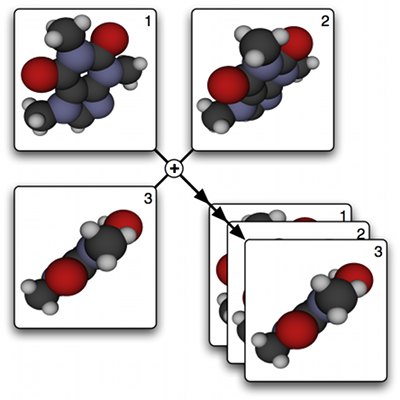
\includegraphics[width=\textwidth]{images/dplex}
  \end{subfigure}
  \begin{subfigure}[b]{0.24\textwidth}
    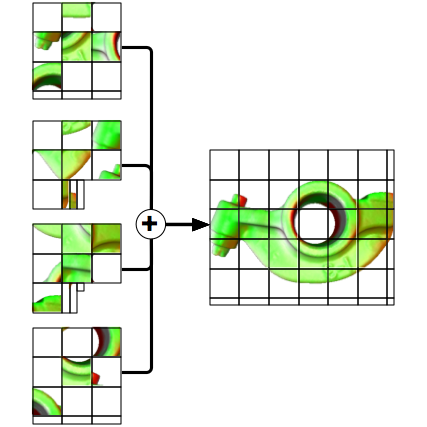
\includegraphics[width=\textwidth]{images/tile}
  \end{subfigure}
  \begin{subfigure}[b]{0.24\textwidth}
    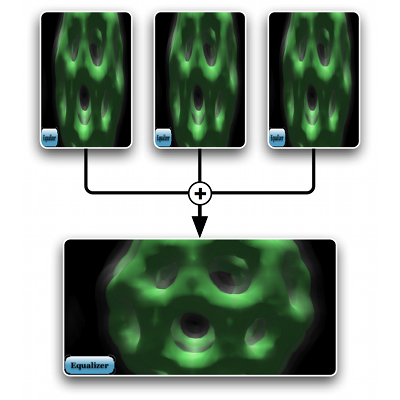
\includegraphics[width=\textwidth]{images/pixel}
  \end{subfigure}
  \begin{subfigure}[b]{0.24\textwidth}
    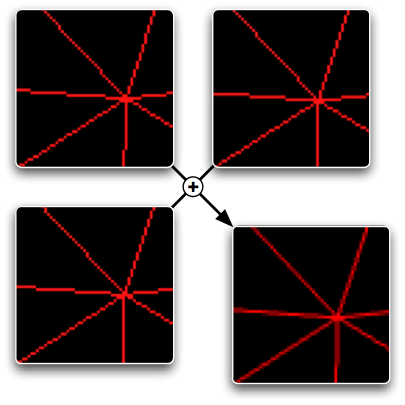
\includegraphics[width=\textwidth]{images/subpixel}
  \end{subfigure}\\[\medskipamount]
  \begin{subfigure}[t]{0.24\textwidth}
    {\tiny\begin{lstlisting}
compound {
  channel "destination"
  framerate_equalizer {}
  compound {
    channel "source1"
    phase 0 period 3
    outputframe  { name "frame" }
  }
  compound {
    channel "source2"
    phase 1 period 3
    outputframe  { name "frame" }
  }
  compound {
    channel "source3"
    phase 2 period 3
    outputframe  { name "frame" }
  }
  inputframe { name "frame" }
}
    \end{lstlisting}\vspace{24ex}}
    \caption{\label{fig:dplex}Time-Multiplex}
  \end{subfigure}
  \begin{subfigure}[t]{0.24\textwidth}
    {\tiny\begin{lstlisting}
compound {
  channel "destination"
  outputtiles {
    name "queue"
    size [ 64 64 ]
  }
  compound {
    channel "destination"
    inputtiles { name "queue" }
  }
  compound {
    channel "source1"
    inputtiles { name "queue" }
    outputframe {}
  }
  compound {
    channel "source2"
    inputtiles { name "queue" }
    outputframe {}
  }
  compound {
    channel "source3"
    inputtiles { name "queue" }
    outputframe {}
  }
  inputframe { name "frame.source1" }
  inputframe { name "frame.source2" }
  inputframe { name "frame.source3" }
}
    \end{lstlisting}}
    \caption{\label{fig:tiles}Tiles}
  \end{subfigure}
  \begin{subfigure}[t]{0.24\textwidth}
    {\tiny\begin{lstlisting}
compound {
  channel "dest"
  compound {
    channel "dest"
    pixel [ 0 0 3 1 ]
    outputframe { type texture }
  }
  compound {
    channel "source1"
    pixel [ 1 0 3 1 ]
    outputframe {}
  }
  compound {
    channel "source2"
    pixel [ 2 0 3 1 ]
    outputframe {}
  }
  inputframe { name "frame.dest" }
  inputframe { name "frame.source1" }
  inputframe { name "frame.source2" }
}
    \end{lstlisting}\vspace{21ex}}
    \caption{\label{fig:pixel}Pixel}
  \end{subfigure}
  \begin{subfigure}[t]{0.24\textwidth}
    {\tiny\begin{lstlisting}
compound {
  channel "dest"
  compound {
    channel "dest"
    subpixel [ 0 3 ]
    outputframe { type texture }
  }
  compound {
    channel "source1"
    subpixel [ 1 3 ]
    outputframe {}
  }
  compound {
    channel "source2"
    subpixel [ 1 3 ]
    outputframe {}
  }
  inputframe { name "frame.dest" }
  inputframe { name "frame.source1" }
  inputframe { name "frame.source2" }
}
    \end{lstlisting}\vspace{21ex}}
    \caption{\label{fig:subpixel}Subpixel}
  \end{subfigure}
  \caption{New \textsf{Equalizer} task decomposition modes and their compound
descriptions for parallel rendering}
  \label{fig:compounds}
\end{figure*}


\subsubsection{Time-Multiplex}

Time-multiplexing (\fig{fig:dplex}), also called AFR or DPlex, was first
implemented in \cite{BRE:05} for shared memory machines. It is however a better
fit for distributed memory systems, since the separate memory space makes
concurrent rendering of different frames easier to implement. While it increases
the framerate linearly, it does not decrease the latency between user input and
the corresponding output. Consequently, this decomposition mode is mostly useful
for non-interactive movie generation. It is transparent to \textsf{Equalizer}
applications, but does require the configuration latency to be equal or greater
than the number of source channels. Furthermore, to work in multi-threaded,
multi-GPU configurations, the application needs to support running the rendering
threads asynchronously (\sref{sec:threading}). The output frame rate of the
destination channel may be smoothened using a {\em frame rate equalizer}
(\sref{sec:framerateEq}).

\subsubsection{Tiles and Chunks}\label{sec:tile}

Tile (\fig{fig:tiles}) and chunk decompositions are a variant of sort-first and
sort-last rendering, respectively. They decompose the scene into a predefined
set of fixed-size image tiles or database ranges. These tasks, or work packages are queued and
processed by all source channels by polling a server-central queue. Prefetching
ensures that the task communication overlaps with rendering. As shown in~
\cite{SPEP:16}, these modes can provide better performance due to being inherently
load-balanced, as long as there is an insignificant overhead for the render task
setup. This mode is transparent to \textsf{Equalizer} applications.


\subsubsection{Pixel}

Pixel compounds (\fig{fig:pixel}) decompose the destination channel by
interleaving rows or columns in image space. They are a variant of sort-first
decomposition which works well for fill-limited applications which are not
geometry bound, for example direct volume rendering. Source channels cannot
reduce geometry load through view frustum culling, since each source channel has
almost the same frustum. However, the fragment load on all source channels is
reduced linearly and well load-balanced due to the interleaved distribution of
pixels. This functionality is transparent to \textsf{Equalizer} applications,
and the default compositing uses the stencil buffer to blit pixels onto the
destination channel.

\subsubsection{Subpixel}

Subpixel compounds (\fig{fig:subpixel}) are similar to pixel compounds, but they
decompose the work for a single pixel, for example with Monte-Carlo ray tracing,
FSAA or depth of field rendering. Composition typically uses accumulation and
averaging of all computed fragments for a pixel. This feature is not fully
transparent to the application, since it needs to adapt (jitter or tilt) the
frustum based on the iteration executed. Furthermore, subpixel compounds
interact with idle image refinements, e.g., they can accelerate idle
anti-aliasing of a scene when the camera and scene are not changed.

%------------------------------------------------------------------------------
\subsection{Equalizers}

{\em Equalizers} are an addition to compound trees. They modify parameters of
their respective subtree at runtime to dynamically optimize the resource usage,
by each tuning one aspect of the decomposition. Due to their nature, they are
transparent to application developers, but might have application-accessible
parameters to tune their behavior. Resource equalization is the critical
component for scalable parallel rendering, and therefore the eponym for the
\textsf{Equalizer} project name.

\begin{figure*}[ht]\center
  \begin{subfigure}[b]{0.24\textwidth}
    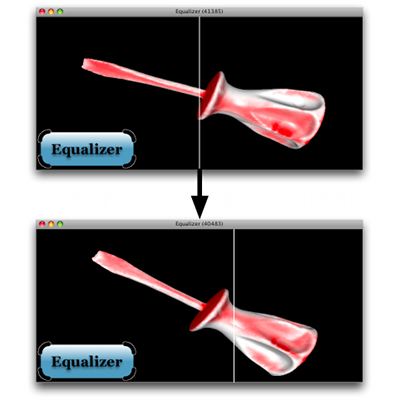
\includegraphics[width=\textwidth]{images/loadeq}
      \caption{\label{fig:loadeq}Load-Balancing}
  \end{subfigure}
  \begin{subfigure}[b]{0.24\textwidth}
    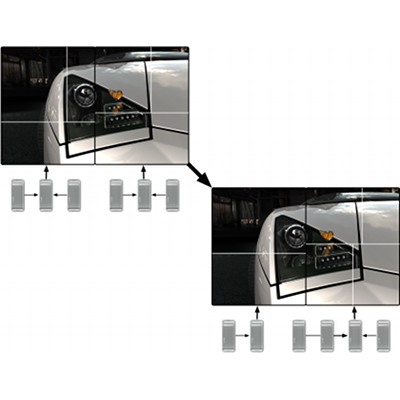
\includegraphics[width=\textwidth]{images/vieweq}
      \caption{\label{fig:vieweq}Cross-Segment Load-Balancing}
  \end{subfigure}
  \begin{subfigure}[b]{0.24\textwidth}
    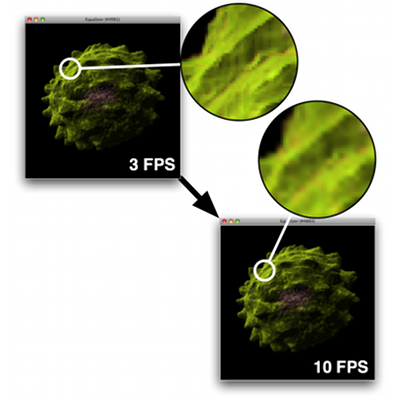
\includegraphics[width=\textwidth]{images/dfr}
      \caption{\label{fig:dfr}Dynamic Frame Resolution}
  \end{subfigure}
  \begin{subfigure}[b]{0.24\textwidth}
    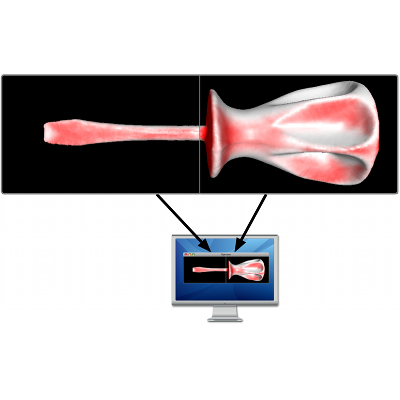
\includegraphics[width=\textwidth]{images/monitoreq}
      \caption{\label{fig:monitor}Monitoring}
  \end{subfigure}
  \caption{Runtime modifications}
  \label{fig:equalizers}
\end{figure*}

\subsubsection{Sort-First and Sort-Last Load Balancing}

Sort-first (\fig{fig:loadeq}) and sort-last load balancing are the most obvious
optimizations for these parallel rendering modes. Our load equalizers are fully
transparent for application developers; that is, they use a reactive approach
based on past rendering times. This assumes a reasonable frame-to-frame
coherency. Equalizer implements two different algorithms, a
\textsf{load\_equalizer} and a \textsf{tree\_equalizer}. The result section
provides some evidence on the strengths and weaknesses of both algorithms.

The \textsf{load\_equalizer} stores a 2D or 1D grid of the load, mapping the
load of each channel. The load is stored in normalized 2D/1D coordinates using
$\frac{time}{area}$ as the load, the contributing source channels are organized
in a binary tree, and then the algorithm balances the two branches of each level
by equalizing the integral over the cost area map on each side.

The \textsf{tree\_equalizer} also uses a binary tree for recursive load
balancing. It computes the accumulated render time on all nodes of the tree, and
uses this to allocate an equal render time to each subtree. It makes no
assumption of the load distribution in 2D or 1D space, it only tries to correct
the imbalance in render time.

We have implemented various tunable parameters for both equalizers allowing
application developers to optimize the load balancing based on the
characteristics of their rendering algorithm:

\begin{compactdesc}
\item[Split Mode] configures the tile layout: horizontal or vertical stripes,
and 2D, a binary tree split alternating the split axis on each level, resulting
in compact 2D tiles.
\item[Damping] reduces frame-to-frame oscillations. The equal load distribution
within the region of interest assumed by the load equalizer is in reality not
equal, causing the load balancing to overshoot. Damping is a normalized scalar
defining how much of the computed delta from the previous position is applied to
the new split.
\item[Resistance] eliminates small deltas in the load balancing step. This might
help the application to cache visibility computations since the frustum does not
change each frame.
\item[Boundaries] define the modulo factor in pixels onto which a load split may
fall. Some rendering algorithms produce artefacts related to the OpenGL raster
position, e.g., screen door transparency, which can be eliminated by aligning
the boundary to the pixel repetition. Furthermore, some rendering algorithms are
sensitive to cache alignments, which can again be exploited by chosing the
corresponding boundary.
\end{compactdesc}

\subsubsection{Cross-Segment Load Balancing}

Cross-segment load balancing (\fig{fig:vieweq}) addresses the optimal resource
allocation of $n$ rendering resources to $m$ output channels (with $n\geq m$). A
view equalizer works in conjunction with load equalizers balancing the
individual output channels. It monitors the usage of shared source channels
across outputs and activates them to balance the rendering time of all outputs.
In \cite{EEP:11}, we provide a detailed description and evaluation of our
algorithm.

\subsubsection{Dynamic Frame Resolution}

The DFR equalizer (\fig{fig:dfr}) provides a functionality similar to dynamic
video resizing \cite{MBDM:97}, that is, it maintains a constant framerate by
adapting the rendering resolution of a fill-limited application. In
\textsf{Equalizer}, this works by rendering into a source channel (typically on
a FBO) separate to the destination channel, and then scaling the rendering
during the transfer (typically through an on-GPU texture) to the destination
channel. The DFR equalizer monitors the rendering performance and accordingly
adapts the resolution of the source channel and zoom factor for the source to
destination transfer. If the performance and source channel resolutions allows,
this will not only subsample, but also supersample the destination channel to
reduce aliasing artefacts.

\subsubsection{Frame Rate Equalizer}\label{sec:framerateEq}

The framerate equalizer smoothens the output frame rate of a destination channel
by instructing the corresponding window to delay its buffer swap to a minimum
time between swaps. This is regularly used for time-multiplexed decompositions,
where source channels tend to drift and finish their rendering unevenly
distributed over time. This equalizer is however fully independent of DPlex
compounds, and may be used to smoothen irregular application rendering
algorithms.

\subsubsection{Monitoring}

The monitor equalizer (\fig{fig:monitor}) allows to reuse the rendering on
another channel, typically for monitoring a larger setup on a control
workstation. Output frames on the display channels are connected to input frames
on a single monitoring channel. The monitor equalizer changes the scaling factor
and offset between the output and input, so that the monitor channel has the
same, but typically downscaled view, as the originating segments.

%------------------------------------------------------------------------------
\subsection{Optimizations}

\subsubsection{Region of Interest}

The region of interest is the screen-space 2D bounding box enclosing the
geometry rendered by a single resource. We have extended the core parallel
rendering framework to use an application-provided ROI to optimize the load
equalizer as well as image compositing performance. The load equalizer uses the
ROI to refine its load grid to the regions containing data. The compositing code
uses the ROI to minimize image readback and network transmission. In
\cite{MEP:10} and \cite{EBAHMP:12}, we provide the details of the algorithm, and
show that using ROI can quadruple the rendering performance, in particular for
the costly compositing step in sort-last rendering.

\subsubsection{Asynchronous Compositing}

Asynchronous compositing pipelines rendering with compositing operations, by
executing the image readback, network transfer and image assembly from threads
running in parallel to the rendering threads. In \cite{EBAHMP:12}, we provide
the details of the implementation and experimental data showing an improvement
of the rendering performance of over 25\% for large node counts.

\subsubsection{Download and Compression Plugins}

Compression for the compositing step in parallel rendering is critical for
performance. This not only applies to the well-researched network transfer step,
but also for the transfer between GPU and CPU. \textsf{Equalizer} supports a
variety of
compression algorithms, from very fast RLE encoding, YUV
subsampling on the GPU to JPEG compression. These algorithms are implemented as
runtime-loaded
plugins, allowing easy extension and customization to application-specific
compression. In \cite{MEP:10}, we show this to be a critical step for
interactive performance at scale.

\subsubsection{Thread Synchronization Modes}\label{sec:threading}

Different applications have different degrees on how decoupled and thread-safe
the rendering code is from the application logic. For full decoupling all
mutable data has to have a copy in each render thread, which is not feasible in
many complex applications and large data scenarios. To easily customize the
synchronization of all threads on a single process, \textsf{Equalizer}
implements three threading modes:  Full synchronization, draw synchronization
and asynchronous. Note that the execution between node processes is always
asynchronous, for up to \textsf{latency} frames.

In full synchronization, all threads always execute the same frame; that is, the
render threads are unlocked after \textsf{Node::frameStart}, and the node is
blocked for all render threads to finish the frame before executing
\textsf{Node::frameFinish}. This allows the render threads to read shared data
from all their operations, but provides the slowest performance.

In draw synchronization, the node thread and all render threads are synchronized
for all \textsf{frameDraw} operations; that is, \textsf{Node::frameFinish} is
executed after the last channel is done drawing. This allows the render threads
to read shared data during their draw operation, but not during compositing.
Since compositing is typically independent of the rendered data, this is the
default mode. This mode allows to overlap compositing with rendering and data
synchronization on multi-GPU machines.

In asynchronous execution, all threads run asynchronously. Render threads may
work on different frames at any given time. This mode is the fastest, and
requires the application to have one instance of each mutable object in each
render thread. It is required for using time-multiplex compounds in
multithreaded rendering.

%------------------------------------------------------------------------------
\section{Virtual Reality Features}
%------------------------------------------------------------------------------

Virtual Reality is an important field for parallel rendering. It does however
require special attention to support it as a first-class citizen in a generic
parallel rendering framework. \textsf{Equalizer} has been used in many virtual
reality installations, such as the Cave2 \cite{FNTTL:13}, the high-resolution C6
CAVE at the KAUST visualization laboratory, and head-mounted displays
(\fig{FIG_teaser}). In the following we lay out the features needed to support
these installations, motivated by application use cases.

%------------------------------------------------------------------------------
\subsection{Head Tracking}

Head tracking is the minimal feature needed to support immersive installations.
\textsf{Equalizer} does support multiple, independent tracked views through the
observer abstraction (\sref{sec:observer}). Built-in VRPN support enables the
direct, application-transparent configuration of a VRPN tracker device.
Alternatively, an application can provide a $4\times 4$ tracking matrix defining
the transformation from the canvas coordinate system to the observer. Both
CAVE-like tracking with fixed projection surfaces and HMD tracking with moving
displays are implemented.

%------------------------------------------------------------------------------
\subsection{Dynamic Focus Distance}

To our knowledge, all parallel rendering systems have the focal plane coincide
with the physical display surface. For better viewing comfort, we introduce a
new dynamic focus mode, where the application defines the distance of the focal
plane from the observer, based on the current view direction of the user.
Initial experiments show that this provides better viewing comfort, in
particular for objects placed in front of the physical displays.

%------------------------------------------------------------------------------
\subsection{Asymmetric Eye Position}

Traditional head tracking computes the left and right eye positions by using a
configurable interocular distance. However, human heads are not symmetric, and
by measuring individual users a more precise frustum can be computed.
\textsf{Equalizer} supports this through the optional configuration (file or
programmatically) of individual 3D translations for all eyes relative to the
tracking matrix.

%------------------------------------------------------------------------------
\subsection{Model Unit}

This feature allows applications to specify a scaling factor between the model
and the real world, to allow exploration of macroscopic or microscopic worlds in
virtual reality. The unit is per view, allowing different scale factors within
the same application. It scales both the specified projection surface as well
as the eye position (and therefore separation) to achieve the necessary effect.

%------------------------------------------------------------------------------
\subsection{Runtime Stereo Switch}

Applications can switch each view between mono and stereo rendering at runtime,
and run both monoscopic and stereoscopic views concurrently (\fig{FIG_teaser}
(b)). This switch does potentially involve the start and stop of resources and
processes for passive stereo or stereo-dependent task decompositions
(\sref{sec:reconfig}).

%------------------------------------------------------------------------------
\section{Usability Features}
%------------------------------------------------------------------------------

In this section we present features motivated by real-world application use
cases, i.e., new functionalities rather then performance improvements. We
motivate the use case, explain the architecture and integration into our
parallel rendering framework, and, where applicable, show the steps needed to
use this functionality in applications.

%------------------------------------------------------------------------------
\subsection{Physical and Logical Visualization Setup}

Real-world visualization setups can be complex. An abstract representation of
the display system simplifies the configuration process. Applications often have
the need to be aware of spatial relationship of the display setup, for example
to render 2D overlays or to configure multiple views on a tiled display wall.

We addressed this need through a new configuration section interspersed between
the node/pipe/window/channel hardware resources and the compound trees
configurating the resource usage for parallel rendering.

A typical installation consists of one projection canvas, which is one
aggregated projection surface, e.g., a tiled display wall or a CAVE. Desktop
windows are considered a canvas. Each canvas is made of one or more segments,
which are the individual outputs connected to a display or projector. Segments
can be planar or non-planar to each other, and can overlap or have gaps between
each other. A segment is referencing a channel, which defines the output area of
this segment, e.g., on a DVI connector connected to a projector. This
abstraction covers all use cases from simple windows, tiled display walls with
bezels, to non-planar immersive systems with edge-blending.

A canvas can define a frustum, which will create default, planar sub-frusta for
all of its segments. A segment can also define a frustum, which overrides the
canvas frustum, e.g., for non-planar setups such as CAVEs or curved screens.
These frusta describe a physically-correct display setup for a Virtual Reality
installation. \label{sec:swap} A canvas may have a software or hardware swap
barrier, which will synchronize the rendering of all contributing GPUs. The
software barrier executes a \textsf{glFinish} to ensure the GPU is ready to
swap, a \textsf{Collage} barrier (\sref{sec:barrier}) to synchronize all
segments, the swap buffers call followed by a \textsf{glFlush} to ensure timely
execution of the swap command. The hardware swap barrier is implemented using a
\textsf{NV\_swap\_group} extension.

On each canvas, the application can display one or more views. A view is used in
the sense of the MVC pattern. The view class is available to applications to
define view-specific data for rendering, e.g., a scene, viewing mode or camera.
The application process manages this data, and the render clients receive it for
rendering.

A layout groups one or more views which logically belong together. A layout is
applied to a canvas. The layout assignment can be changed at run-time by the
application. The intersection between views and segments defines which output
channels are available, and which frustum they should use for rendering. These
output channels are then used as destination channels in a compound. They are
automatically created during configuration.

\label{sec:observer}
An observer looks at one or more views. It is described by the observer position
in the world and its eye separation. Each observer has its own stereo
mode, focus distance and eye positions. This allows to have untracked
views and multiple tracked views, e.g., two HMDs, in the same application.

\begin{figure}[ht]\center
  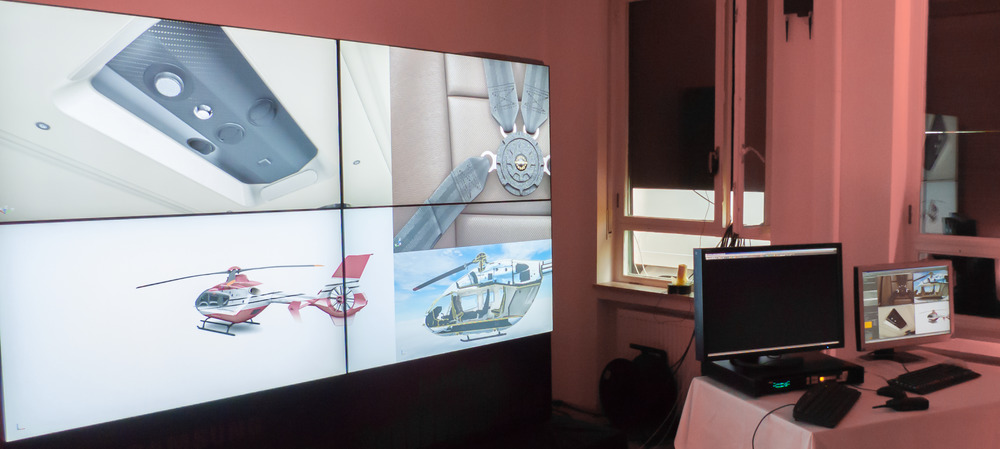
\includegraphics[width=\columnwidth]{images/layout}
  \caption{\label{fLayout}A 2x2 tiled display wall and control host rendering four independent views driven by an eight node visualization cluster}
\end{figure}

\fig{fLayout} shows RTT Deltagen running an example multi-segment, multi-view
setup driven by eight rendering nodes. The main tiled display wall canvas uses
four LCD segments showing one layout with four views, which do not align on the
segment boundaries. This setup creates seven destination channels. The
configuration provides multiple, run-time configurable layouts. It is driven
from the control host on the right, which shows four views, each in their own
canvas and segment windows with a single-view layout each. One view on the
control host synchronizes its content (model and camera) with one view on the
display wall through Collage objects. The control host allows full model
modifications and all workflows supported within the standalone Deltagen
application, and all changes are synchronized to the corresponding rendering
nodes. Since this setup is monoscopic, no head tracking or observers are used.

%------------------------------------------------------------------------------
\subsection{Runtime Reconfiguration}\label{sec:reconfig}

Switching a layout, as described above, or switching the stereo rendering mode,
may involve a different set of resources after the change, including the launch
and exit of render client processes. \textsf{Equalizer} solves this through a
reconfiguration step at the beginning of each rendering frame. Each resource
(channel, window, pipe, node) has an activation count, which is updated when the
layout or any other relevant rendering parameter is changed. When a resource is
found whose activation count does not match its current start/stopped state, the
resource is created or destroyed and \textsf{configInit} or \textsf{configExit}
are called accordingly. In the current implementation, a normal configuration
initialization or exit, as described in \cite{EMP:09}, uses the same code path
with all used resources transitioning to a running or stopped state,
accordingly. Since starting new resources typically requires object mapping and
associated data distribution, it is a costly operation.

%------------------------------------------------------------------------------
\subsection{Automatic Configuration}

Automatic configuration implements the discovery of local and remote resources
as well as the creation of typical configurations using the discovered resources
at application launch time.

The discovery is implemented in a separate library, \textsf{hwsd} (HardWare
Service
Discovery), which uses a plugin-based approach to discover GPUs for GLX, AGL or
WGL windowing systems, as well as network interfaces on Linux, Mac OS X and
Windows. Furthermore, it detects the presence of VirtualGL to allow optimal
configuration of remote visualization clusters. The resources can be discovered
on the local workstation, and through the help of a simple daemon using the
zeroconf protocol, on a set of remote nodes within a visualization cluster. A
session identifier may be used to support multiple users on a single cluster.

The \textsf{Equalizer} server uses the hwsd library to discover local and remote
resources when an hwsd session name instead of a \texttt{.eqc} configuration
file is provided. A set of standard decomposition modes is configured, which can
be selected through activating the corresponding layout.

This versatile mechanism allows non-experts to configure and profit from
multi-GPU workstations and visualization clusters, as well as to provide system
administrators with the tools to implement easy to use integration with cluster
schedulers. This feature is transparent to application developers.

%------------------------------------------------------------------------------
\subsection{Qt Windowing}

Qt is a popular window system with many application developers. Unfortunately,
it imposes a different threading model for window creation and event handling
compared to \textsf{Equalizer}. In \textsf{Equalizer}, each GPU rendering thread
is independently responsible for creating its windows, receiving the events and
eventually dispatching them to the application process main thread. This design
is motivated by the natural threading model of X11 and WGL, and allows simple
sequential semantics between OpenGL rendering and event handling. In contrast,
Qt requires all windows and QOpenGLContext to be created from the Qt main
thread. An existing Qt window or context may subsequently be moved to a
different thread, and events are signalled from the main thread. For Qt windows,
Equalizer will internally dispatch and handle the window creation from the
render to the main thread, move the created objects back to the render thread,
and dispatch Qt signals to the correct render threads.

%------------------------------------------------------------------------------
\subsection{Tide Integration}

\textsf{Tide} (Tiled interactive display environment) is an improved version of
\textsf{DisplayCluster}~\cite{DC}, providing a touch-based, multi-window user
interface for high-resolution tiled display walls. Remote applications receive
input events and send pixel streams using the \textsf{Deflect} client library.
\textsf{Equalizer} includes full support, enabling application-transparent
integration with \textsf{Tide}. When a \textsf{Tide} server is configured, all
output channels of a view stream in parallel to one window on the wall. In
\cite{deflect}, we have shown interactive framerates for a 24 megapixel
resolution over a WAN link. Events received are translated into
\textsf{Equalizer} events and injected into the normal event flow, allowing
seamless application integration.

%------------------------------------------------------------------------------
\subsection{\textsf{Sequel}}\label{sec:sequel}

\textsf{Sequel} is a simplification layer for \textsf{Equalizer}. It is based on
the realization that while fully expressive, the verbatim abstraction layer of
nodes, pipes, windows and channels in \textsf{Equalizer} requires significant
learning to fully understand and exploit. In reality, a higher abstraction of
only \textsf{Application} and \textsf{Renderer} is sufficient for many use
cases. In \textsf{Sequel}, the application class drives the configuration, and
one renderer instance is created for each (pipe) render thread. They also
provide the natural place to store and distribute data. Last, but not least,
\textsf{ViewData} provides a convenient way to manage multiple views by storing
the camera, model or any other view-specific information.


%------------------------------------------------------------------------------
\section{The \textsf{Collage} Network Library}
%------------------------------------------------------------------------------

An important part of writing a parallel rendering application is the
communication layer between the individual processes. \textsf{Equalizer} relies
on the
\textsf{Collage} network library for its internal operation. \textsf{Collage}
furthermore provides
powerful abstractions for writing \textsf{Equalizer} applications, which are
introduced
in this section.

%------------------------------------------------------------------------------
\subsection{Architecture}

\textsf{Collage} provides networking functionality of different abstraction
layers, gradually providing higher level functionality for the programmer. The
main primitives in \textsf{Collage} and their relation are shown in
\fig{fNetObject} and provide:

\begin{compactdesc}
\item[Connection] A stream-oriented point-to-point communication
  line. The connections
  transmit raw data reliably between two endpoints for unicast connections, and
  between a set of endpoints for multicast connections. For unicast,
  process-local pipes, TCP and Infiniband RDMA are implemented. For multicast,
  a reliable, UDP-based protocol is discussed in \sref{sec:RSP}.
\item[DataI/OStream] Abstracts the input and output of C++ data types from or to
  a set of connections by implementing output stream operators. Uses buffering
  to aggregate data for network transmission. Performs endian swapping during
  input if the endianness differs between the originating and local node.
\item[Node and LocalNode] The abstraction of a process in the cluster. Nodes
  communicate with each other using connections. A LocalNode listens on various
  connections and processes requests for a given process. Received data is
  wrapped in ICommands and dispatched to command handler methods. A Node is a
  proxy for a remote LocalNode. The \textsf{Equalizer} Client object is a
LocalNode.
\item[Object] Provides object-oriented, versioned data distribution of C++
  objects between nodes. Objects are registered or mapped on a Local\-Node.
\end{compactdesc}

\begin{figure}[ht]\center
  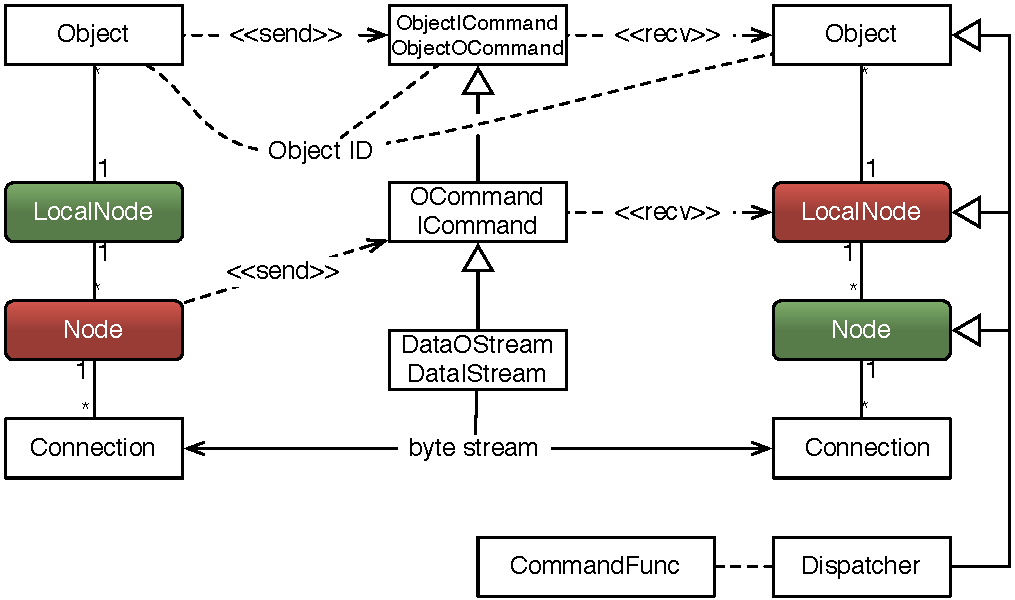
\includegraphics[width=\columnwidth]{images/netObject}
  \caption{\label{fNetObject}Communication between two \textsf{Collage} objects}
\end{figure}

%------------------------------------------------------------------------------
\subsection{Reliable Stream Protocol}\label{sec:RSP}

RSP is an implementation of a reliable multicast protocol over unreliable UDP
transport. RSP behaves similarly to TCP, it provides full reliability and
ordering of the data, and slow receivers will eventually throttle the sender
through a sliding window algorithm. This behavior is needed to guarantee
delivery of data in all situations. Pragmatic generic multicast (PGM~\cite{pgm})
provides full ordering, but slow clients will disconnect from the multicast
session instead of throttling the send rate.

RSP combines various established algorithms~\cite{adamson2004negative,
  Gau:2002:MFC:506824.506832} for multicast in an open source implementation
capable of delivering wire speed transmission rates on high-speed LAN
interfaces. In the following we will outline the RSP protocol and implementation
as well as motivate the design decisions. Any defaults given below are for
Linux or OS X, the Windows UDP stack requires different default values which can
be found in the implementation.

Our RSP implementation uses a separate protocol thread for each RSP group, which
handles all reads and writes on the multicast group. This thread implements the
protocol handling and communicates with the application threads through
thread-safe queues. These queues contain datagrams of the application byte
stream, prefixed by a type-specific header of at most eight bytes. Each
connection has a configurable number of buffers, (1024 by default) of a
configurable MTU (1470 bytes default) which are either free for use or in
transmission.

Handling a smooth packet flow is critical for performance. RSP uses active flow
control to advance the byte stream buffered by the implementation. Each incoming
connection actively acknowledges every $n$ (17 by default) packets fully
received. The incoming connections temporarily offset this acknowledgment by
their connection identifier to avoid bursts of acks. Any missed datagram is
actively nack'ed as soon as it is detected. Write connections continuously
retransmit packets from nack datagrams, and advance their window upon reception
of acks from all readers. Furthermore, the writer will explicitly request an ack
or nack when it runs out of empty buffers or finishes its write queue. Nack
datagrams may contain multiple ranges of missed datagrams, which is motivated by
the observation that UDP implementations often drop multiple packets at once.

Congestion control is necessary to optimize bandwidth usage. While TCP uses the
well-known AIMD (additive increase, multiplicative decrease) algorithm, we have
chosen a more aggressive congestion control algorithm of additive increase and
additive decrease. This has proven experimentally to be more optimal: UDP is
often rate-limited by switches; that is, packets are discarded regularly and not
exceptionally. Only slowly backing of the current send rate helps to stay close
to this limit. Furthermore, our RSP traffic is limited to the local subnet,
making cooparation between multiple data stream less of an issue. Send rate
limiting uses a bucket algorithm, where over time the bucket fills with send
credits, from which sends are substracted. If there are no available credits,
the sender sleeps until sufficient credits are available.

%------------------------------------------------------------------------------
\subsection{Distributed, Versioned Objects}

Adapting an existing application for parallel rendering requires the
synchronization of application data across the processes in the parallel
rendering setup. Existing parallel rendering frameworks address this often
poorly, at best they rely on MPI to distribute data. Real-world, interactive
visualization applications are typically written in C++ and have complex data
models and class hierarchies to represent their application state. As outlined
in \cite{EMP:09}, the parallel rendering code in an \textsf{Equalizer}
application only
needs access to the data needed for rendering, as all application logic is
centralized in the application main thread. We have encountered two main
approaches to address this distribution: Using a shared filesystem for static
data, or using data distribution for static and dynamic data.

Distributed objects are not required to build \textsf{Equalizer} applications.
While most
developers choose to use this abstraction for convenience, we have seen
applications using other means for data distribution, e.g., MPI.

\subsubsection{Programming Interface}

Distributed objects in \textsf{Collage} provide powerful, object-oriented data
distribution for C++ objects. They facilitate the implementation of data
distribution in a cluster environment. Distributed objects are created by
subclassing from \textsf{co::Serializable} or \textsf{co::Object}. The
application programmer implements serialization and deserialization of the
distributed data. Distributed objects can be static (immutable) or
dynamic. Objects have a universally unique identifier (UUID) to address them
cluster-wide. A master-slave model is used to establish mapping and data
synchronization across processes. Typically, the application main loop registers
a master instance and communicates the UUID to the render clients, which map
their instance to the given identifier. The following object types are
available:

\begin{compactdesc}
\item[Static] The object is not versioned nor buffered. The instance data is
  serialized whenever a new slave instance is mapped. No additional data is
  stored.
\item[Instance] The object is versioned and buffered. The instance and delta
  data are identical; that is, only instance data is serialized. Previous
  instance data is saved to be able to map old versions.
\item[Delta] The object is versioned and buffered. The delta data is typically
  smaller than the instance data. The delta data is transmitted to slave
  instances for synchronization. Previous instance and delta data is saved to be
  able to map and sync old versions.
\item[Unbuffered] The object is versioned and unbuffered. No data is stored, and
  no previous versions can be mapped. No old versions can be mapped and no
  additional data is stored.
\end{compactdesc}

All distributed objects have to implement \textsf{getInstanceData} and
\textsf{applyInstanceData} to serialize and deserialize the object's distributed
data. These methods provide an output or input stream as a parameter, which
abstracts the data transmission and can be used like a \textsf{std::stream}.
The data streams implement efficient buffering and compression, and
automatically select the best connection for data transport. Custom data type
serializers can be implemented by providing the appropriate serialization
functions. No pointers should be directly transmitted through the data
streams. For pointers, the corresponding object is typically a distributed
object as well, and its identifier and potentially version is transmitted in
place of the memory address.

Dynamic objects are versioned, and have to override \textsf{getChangeType} to
indicate how they want to have changes to be handled. Upon \textsf{commit} the
delta data from the previous version is sent, if available using multicast, to
all mapped slave instances. The data is queued on the remote node, and is
applied when the application calls \textsf{sync} to synchronize the object to a
new version. The \textsf{sync} method might block if a version has not yet been
committed or is still in transmission. All versioned objects the following
characteristics:

\begin{compactitem}
\item The master instance of the object generates new versions for all
  slaves. These versions are continuous. It is possible to commit on slave
  instances, but special care has to be taken to handle possible
  conflicts.
\item Slave instance versions can only be advanced; that is, \textsf{sync(
  version )} with a version smaller than the current version will fail.
\item Newly mapped slave instances are mapped to the oldest available
  version by default, or to the version specified when calling
  \textsf{mapObject}.
\end{compactitem}

Besides the instance data serialization methods used to map an object, delta and
unbuffered objects may implement \textsf{pack} and \textsf{unpack} to serialize
or deserialize the changes since the last version.

\label{sec:Serializable}The \textsf{Collage} Serializable implements one
convenient usage
pattern for object data distribution. The \textsf{co::Serializable} data
distribution is based on the concept of dirty bits, allowing inheritance with
data distribution. Dirty bits form a 64-bit mask which marks the parts of the
object to be distributed during the next commit. For serialization, the
application developer implements \textsf{serialize} or \textsf{deserialize},
which are called with the bit mask specifying which data has to be transmitted
or received. During a commit or sync, the current dirty bits are given, whereas
during object mapping all dirty bits are passed to the serialization methods.

Blocking commits allow to limit the number of outstanding, queued versions on
the slave nodes. A token-based protocol will block the commit on the master
instance if to many unsynchronized versions exist.

\subsubsection{Optimizations}

The API presented in the previous section provides sufficient abstraction to
implement various optimizations for faster mapping and synchronization of data:
compression, chunking, caching, preloading and multicast. The results section
evaluates these optimizations.

The most obvious one is compression. Recently, many new compression algorithms
have been developed which exploit modern CPU architectures and deliver
compression rates well above one gigabyte per second. \textsf{Collage} uses the
Pression library~\cite{pression}, which provides an unified interface for a
number of compression libraries, such as FastLZ~\cite{jesperfast},
Snappy~\cite{snappy} and ZStandard~\cite{zstd}. It also contains a custom,
virtually zero-cost RLE compressor. Pression parallelizes the compression and
decompression using data decomposition. This compression is generic, and
implemented transparently for the application. Applications can also use
data-specific compression.

The data streaming interface also implements chunking, which aims to pipeline
the serialization code with the network transmission. After a configurable
number of bytes has been serialized to the internal buffer, it is transmitted
and serialization continues. This is used both for the initial mapping data and
for commit data.

Caching retains instance data of objects in a cache, and reuses this data to
accelarate mapping of objects. The instance cache is either filled by
``snooping'' on multicast transmissions or by an explicit preloading when the
master objects are registered. The preloading (``send on register'') sends
instance data of recently registered master objects while the correspinding node
is idle to all connected nodes. These nodes simply enter the received data to
their cache. Preloading uses multicast when available.

Due to the master-slave model of data distribution, multicast can be used to
optimize the transmission time of data. If the contributing nodes share a
multicast session, and more than one slave instance is mapped, \textsf{Collage}
automatically uses the multicast connection to send the new version
information.

%------------------------------------------------------------------------------
\subsection{Barriers, Queues and Object Maps}\label{sec:barrier}

\textsf{Collage} implements a few generic distributed objects which are used by
\textsf{Equalizer}
and applicatons. A barrier is a distributed barrier primitive used for software
swap barriers in \textsf{Equalizer} (\sref{sec:swap}). Its implementation
follows a
simple master-slave approach, which has shown to by sufficient for this use
case. Queues are single producer, multiple consumer FIFOs. To hide network
latencies, the consumers use prefetching of queue items into a local queue. They
are used for tile and chunk compounds (\sref{sec:tile}).

The object map facilitates distribution and synchronization of a collection of
distributed objects. Master versions can be registered on a central node, e.g.,
the application node in \textsf{Equalizer}. Consumers, e.g., \textsf{Equalizer}
render clients,
can selectively map the objects they are interested in. Committing the object
map will commit all registered objects and sync their new version to the
slaves. Syncing the map on the slaves will synchronize all mapped instances to
the new version recorded in the object map. This effective design allows data
distribution with minimal application logic. It is used by \textsf{Sequel}
(\sref{sec:sequel}) and other \textsf{Collage} applications.

%----------------------------------------------------------------------
\section{Example Applications} \label{sApplications}
%----------------------------------------------------------------------

In this section, we present some major applications built using
\textsf{Equalizer}, and
show how they interact with the framework to solve complex parallel rendering
problems.

%------------------------------------------------------------------------------
\subsection{Livre}

Livre (Large-scale Interactive Volume Rendering Engine) is a GPU ray-casting based parallel
4D volume renderer, implementing state-of-the-art view-dependent level-of-detail rendering (LOD)
and out-of-core data management~\cite{EHKRW:06}. Hierarchical and out-of-core LOD
data management is supported by an implicit volume octree, accessed asynchronously
by the renderer from a data source on a shared file system. Different data sources providing
an octree conform access to RAW or compressed as well as to implicitly generated volume data
(e.g. such as from event simulations or surface meshes) can be used.

High-level state information, e.g., camera position and rendering settings, is shared in Livre
through \textsf{Collage} objects between the parallel applications and rendering threads.
Sort-first decomposition is efficiently supported through octree traversal and culling both
for scalability as well as for driving large-scale tiled display walls.

%------------------------------------------------------------------------------
\subsection{RTT Deltagen}

RTT Deltagen (now Dassault 3D Excite) is a commercial application for
interactive, high quality rendering of CAD data. The RTT Scale module,
delivering multi-GPU and distributed execution, is based on \textsf{Equalizer}
and \textsf{Collage}, and has driven many of the aforementioned features.

RTT Scale uses a master-slave execution mode, were a single running Deltagen
instance can go into ``Scale mode'' at any time by launching an
\textsf{Equalizer} configuration. Consequently, the whole internal
representation needed for rendering is based on a \textsf{Collage}-based data
distribution. The rendering clients are separate, smaller applications which
will map their scenes during startup. At runtime, any change performed in the
main application is committed as a delta at the beginning of the next frame,
following a design pattern similar to the \textsf{Collage Serializable}
(\sref{sec:Serializable}). Multicast (\sref{sec:RSP}) is used to keep data
distribution times during session launch reasonable for larger cluster sizes
(tens to hundreds of nodes).

RTT Scale is used for a wide variety of use cases. In virtual reality, the
application is used for virtual prototyping and design reviews in front of
high-resolution display walls and CAVEs, as well as for virtual prototyping of
human-machine interactions CAVEs and HMDs (\fig{FIG_teaser}(b)). For
scalability, sort-first and tile compounds are used to achieve fast,
high-quality rendering, primarily for interactive raytracing, both based on CPUs
and GPUs. For CPU-based raytracing, often Linux-based rendering clients are used
with a Windows-based application node.

%------------------------------------------------------------------------------
\subsection{RTNeuron}

RTNeuron \cite{HBBES:13} is a scalable real-time rendering tool for the
visualisation of neuronal simulations based on cable models. It is on
OpenSceneGraph for data management and Equalizer for parallel rendering, and
focuses not only on fast rendering times, but also on fast loading times with no
offline preprocessing. It provides level of detail (LOD) rendering, high quality
anti-aliasing based on jittered frusta and accumulation during still views,
interactive modification of the visual representation of neurons in a per-neuron
basis (full neuron vs. soma only, branch pruning depending on the branch level,
\dots). RTNeuron implements both sort-first and sort-last rendering with order
independent transparency.

%------------------------------------------------------------------------------
\subsection{RASTeR}

RASTeR~\cite{BGP:09} is an out-of-core and view-dependent real-time multiresolution
terrain rendering approach using a patch-based restricted quadtree triangulation.
For load-balanced parallel rendering~\cite{GMBP:10} it exploits fast hierarchical
view-frustum culling of the level-of-detail (LOD) quadtree for sort-first decomposition, and
uniform distribution of the visible LOD triangle patches for sort-last decomposition.
The latter is enabled by a fast traversal of the patch-based restricted quadtree
triangulation hierarchy which results in a list of selected LOD nodes,
constituting a view-dependent cut or \emph{front of activated nodes} through the LOD hierarchy.
Assigning and distributing equally sized segments of this active LOD front to the concurrent
rendering threads results in a near-optimal sort-last decomposition for each frame.

%------------------------------------------------------------------------------
\subsection{Bino}

Bino is a stereoscopic 3D video player capable of running on very large display
systems. Originally written for the immersive semi-cylindrical projection
system at the University of Siegen, it has been used in many installations
thanks to its flexibility of configuration. Bino decodes the video on each
Equalizer rendering process, and only synchronizes the time step globally,
therefore providing a scalable solution to video playback.

%------------------------------------------------------------------------------
\subsection{Omegalib}

Omegalib \cite{Omegalib} is a software framework built on top of Equalizer that
facilitates application development for hybrid reality environments such as the
Cave 2. Hybrid reality enviroments aim to create a seamless 2D/3D environment
that supports both information-rich analysis (traditionally done on tiled
display wall) as well as virtual reality simulation exploration (traditionally
done in VR systems) at a resolution matching human visual acuity. Omegalib
supports dynamic reconfigurability of the display environment, so that areas of
the display can be interactively allocated to 2D or 3D workspaces as needed. It
makes it possible to have multiple immersive applications running on a
cluster-controlled display system, have different input sources dynamically
routed to applications, and have rendering results optionally redirected to a
distributed compositing manager. Omegalib supports pluggable front-ends, to
simplify the integration of third-party libraries like OpenGL, OpenSceneGraph,
and the Visualization Toolkit (VTK).

%----------------------------------------------------------------------
\section{Experimental Results}\label{sec:results}
%----------------------------------------------------------------------

This section presents new experiments, complementing the results of previous
publications~\cite{EP:07, EMP:09, MEP:10, EEP:11, EBAHMP:12, HBBES:13, deflect,
  SPEP:16}. The first part summarizes rendering performance over all
decomposition modes with a few representative workloads. The second part
analyses data distribution performance, in particular how the various
optimizations in \textsf{Collage} effect complex operations in realistic
scenarios.

%------------------------------------------------------------------------------
\subsection{Decomposition Modes}

% Time to render a 4k, 32-step MSAA image of the 1mm David model and Livre using 1 to 10 nodes with all modes (2D, 2D LB, DB, DPlex (over AA steps), tiles, chunks, pixel, subpixel) (+DFR for Livre).

We conducted performance benchmarks for the decomposition modes on a cluster using hexacore Intel Xeon E5-2620v3 CPUs (2.4GHz), 16 GB main memory, 4 GBit/s Ethernet and QDR Infiniband. GCC 4.8 has been used with CMake 3.7 release mode settings to compile the software stack.

We tested the decomposition modes with both volume (\fig{fBenchmarkEVolve}) and polygonal data  (\fig{fBenchmarkEqPly}) and used test scenes that allowed us to finely adjust the rendering load the system has to cope with. In both cases the scene comprised of two rows of instantiated, identical models (the 1mm David model when rendering polygonal data, the $1024^3$ Flower model when rendering volumes), with 30 models in total. Rendering was performed
% with the \textsf{Equalizer} example applications eqPly (for meshes) and eVolve (for volumes)
at 2560x1440. The camera is initially placed in the center of the scene, between the two rows (\fig{fBenchmarkEVolve} and \fig{fBenchmarkEqPly}), rendering only half of the model instances. It is then moved backward over the duration of 800 frames, steadily increasing the rendering load by revealing more models, until all 30 instances are visible.

We investigated the scalability of individual decomposition modes by running the same experiment using a varying number of render nodes (2-9), as well as one dedicated application/display node. We subsequently summed up the duration of all rendered frames for each run (\fig{fCompounds}).

In the case of volume rendering we also measured the performance of decomposition modes under heterogeneous load, which was easily achievable by varying the number of volume samples used for each fragment (1-7), while rendering. This allowed for a consistent linear scaling of rendering load, which was randomly varied (\fig{fEqualizers}) either per frame or per node. Such a linear scaling of load per node corresponds to a scaling of resources, e.g., doubling the rendering load on a specific node corresponds to halving its available rendering resources. To the system this node would then contribute the value 0.5 in terms of {\em normalized compute resources}, as illustrated by \fig{fEqualizers} (left).

This figure gives an impression of how individual modes perform on heterogeneous systems. In this case the tree equalizer performs best (\fig{fEqualizers} (left)), as it allows us to a priori define how much {\em usage} it should make of individual nodes, i.e., bias the allocation of rendering time, in accordance with the expected load / the available compute resources. \fig{fEqualizers} (right), on the other hand, illustrates how the tested decomposition modes perform on a system where compute resources fluctuate randomly every frame, as can arguably be the case for, e.g., cloud-based applications. \FIXME{Should we only mention this in discussion?} For this scenario tile equalizer seems best suited, as it performs load balancing implicitly and does not assume coherence of available resources between frames.

\begin{figure}[ht]\center
  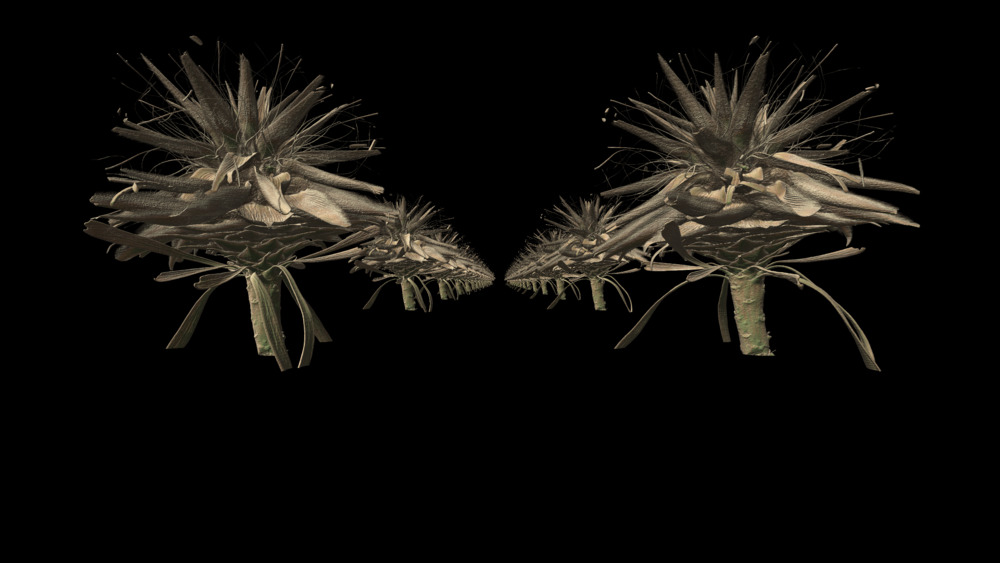
\includegraphics[width=.9\columnwidth]{images/benchmark_eVolve}
  \caption{\label{fBenchmarkEVolve} Benchmarking decomposition modes with Flower volume model at $1024^3$ unsigned byte (1GB).}
\end{figure}

\begin{figure}[ht]\center
  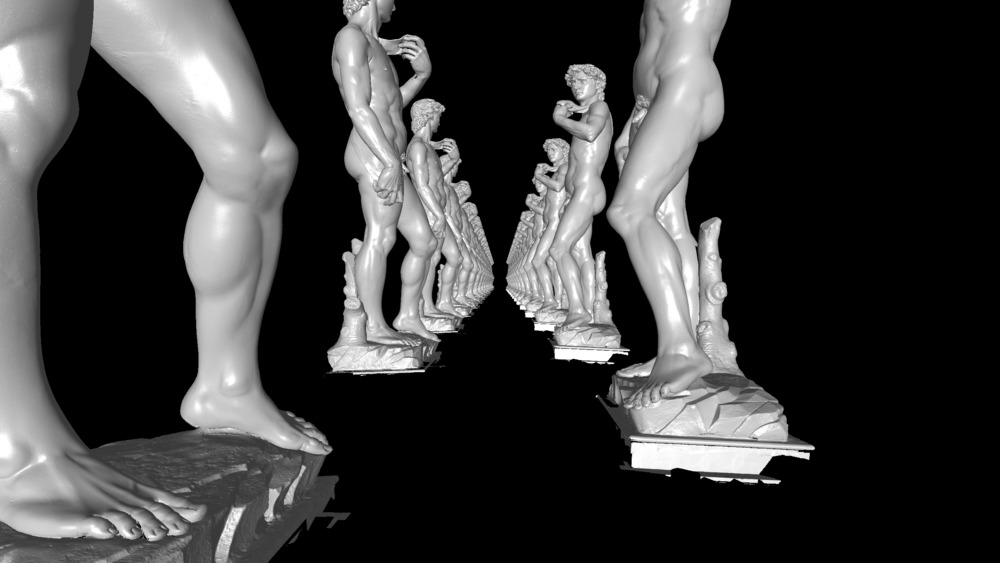
\includegraphics[width=.9\columnwidth]{images/benchmark_eqPly2}
  \caption{\label{fBenchmarkEqPly} Benchmarking decomposition modes with David statue at 1mm resolution (988MB).}
\end{figure}

%------------------------------------------------------------------------------
\subsection{Object Distribution}

The data distribution benchmarks have been performed on a cluster using
dual processor Intel Xeon X5690 CPUs (3.47GHz), 24 GB main memory, 10GBit/s
Ethernet and QDR Infiniband. Intel ICC 2017 has been used with CMake 3.2 release
mode settings to compile the software stack.

To benchmark the data distribution we used two datasets: The David statue at 2mm
resolution (\fig{fDavid2mm}) and 3D volumes of spike frequencies of an
electrical simulation of three million neurons (\fig{fVolumes}).

\begin{figure}[ht]\center
  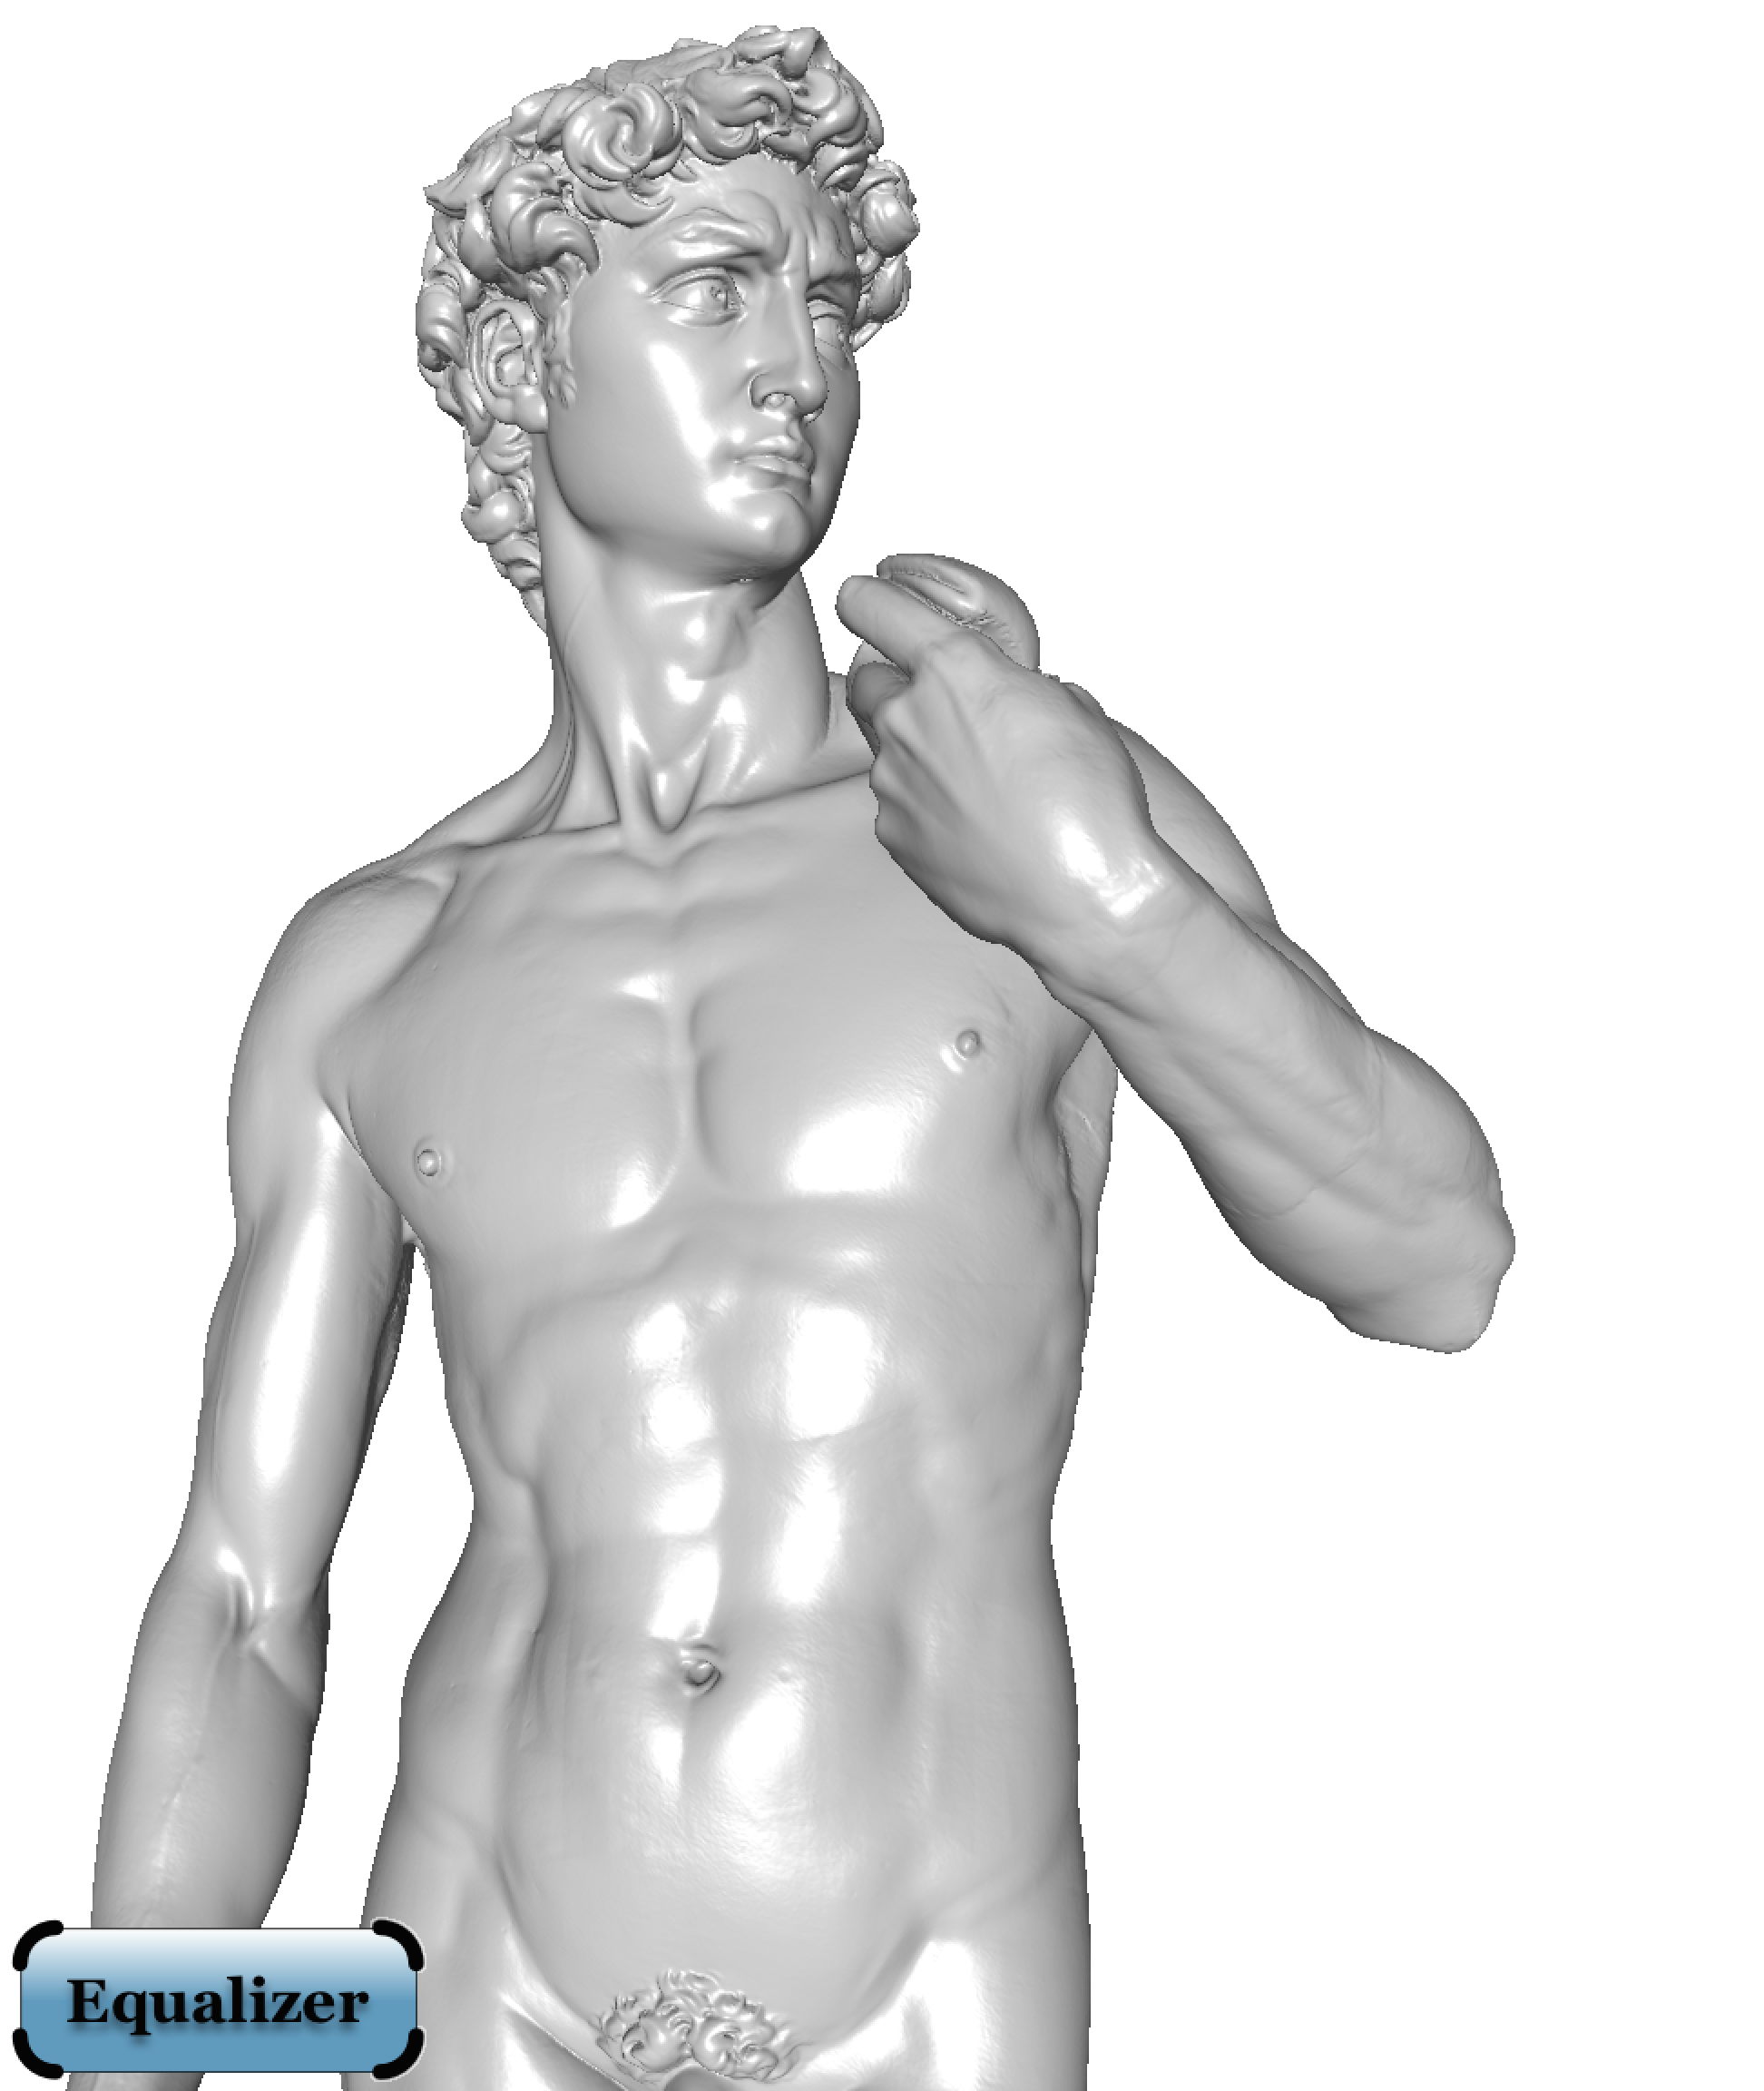
\includegraphics[width=.49\columnwidth]{images/david2mm}
  \caption{\label{fDavid2mm}David statue at 2mm resolution (145MB)}
\end{figure}

The ply file is converted into a kd-Tree for fast view frustum culling and
rendering, and the resulting data structure is serialized in binary form for
data transmission.

\begin{figure}[ht]\center
  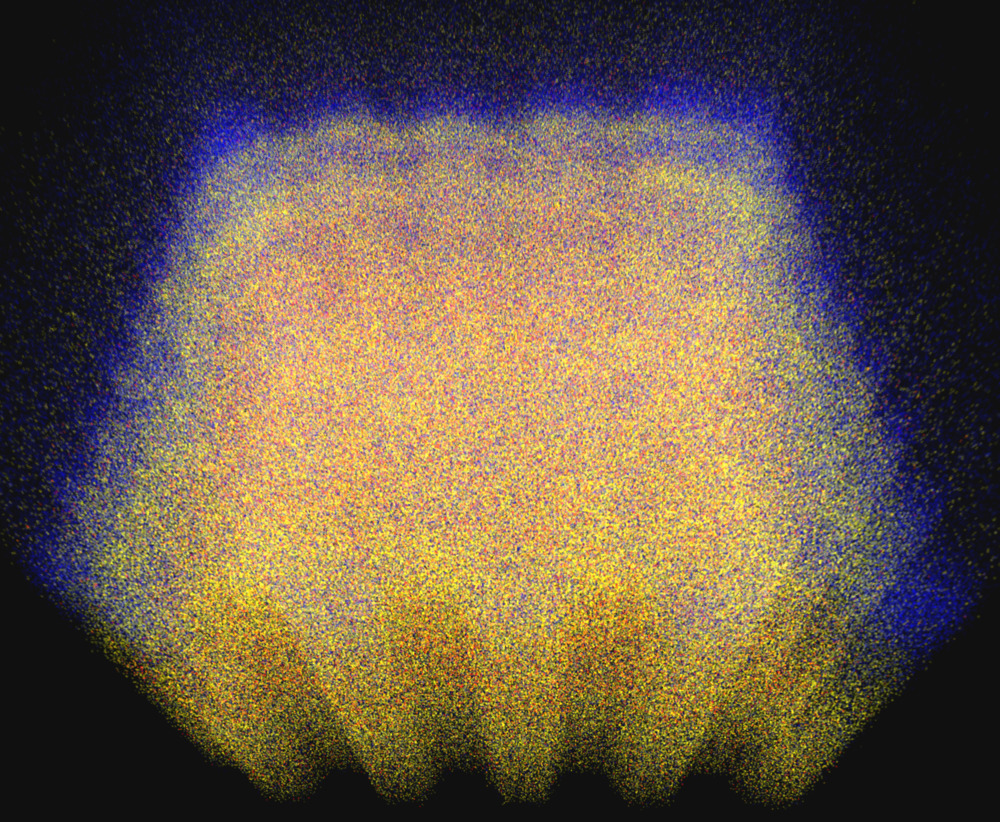
\includegraphics[height=.44\columnwidth]{images/spikes512}\hfil
  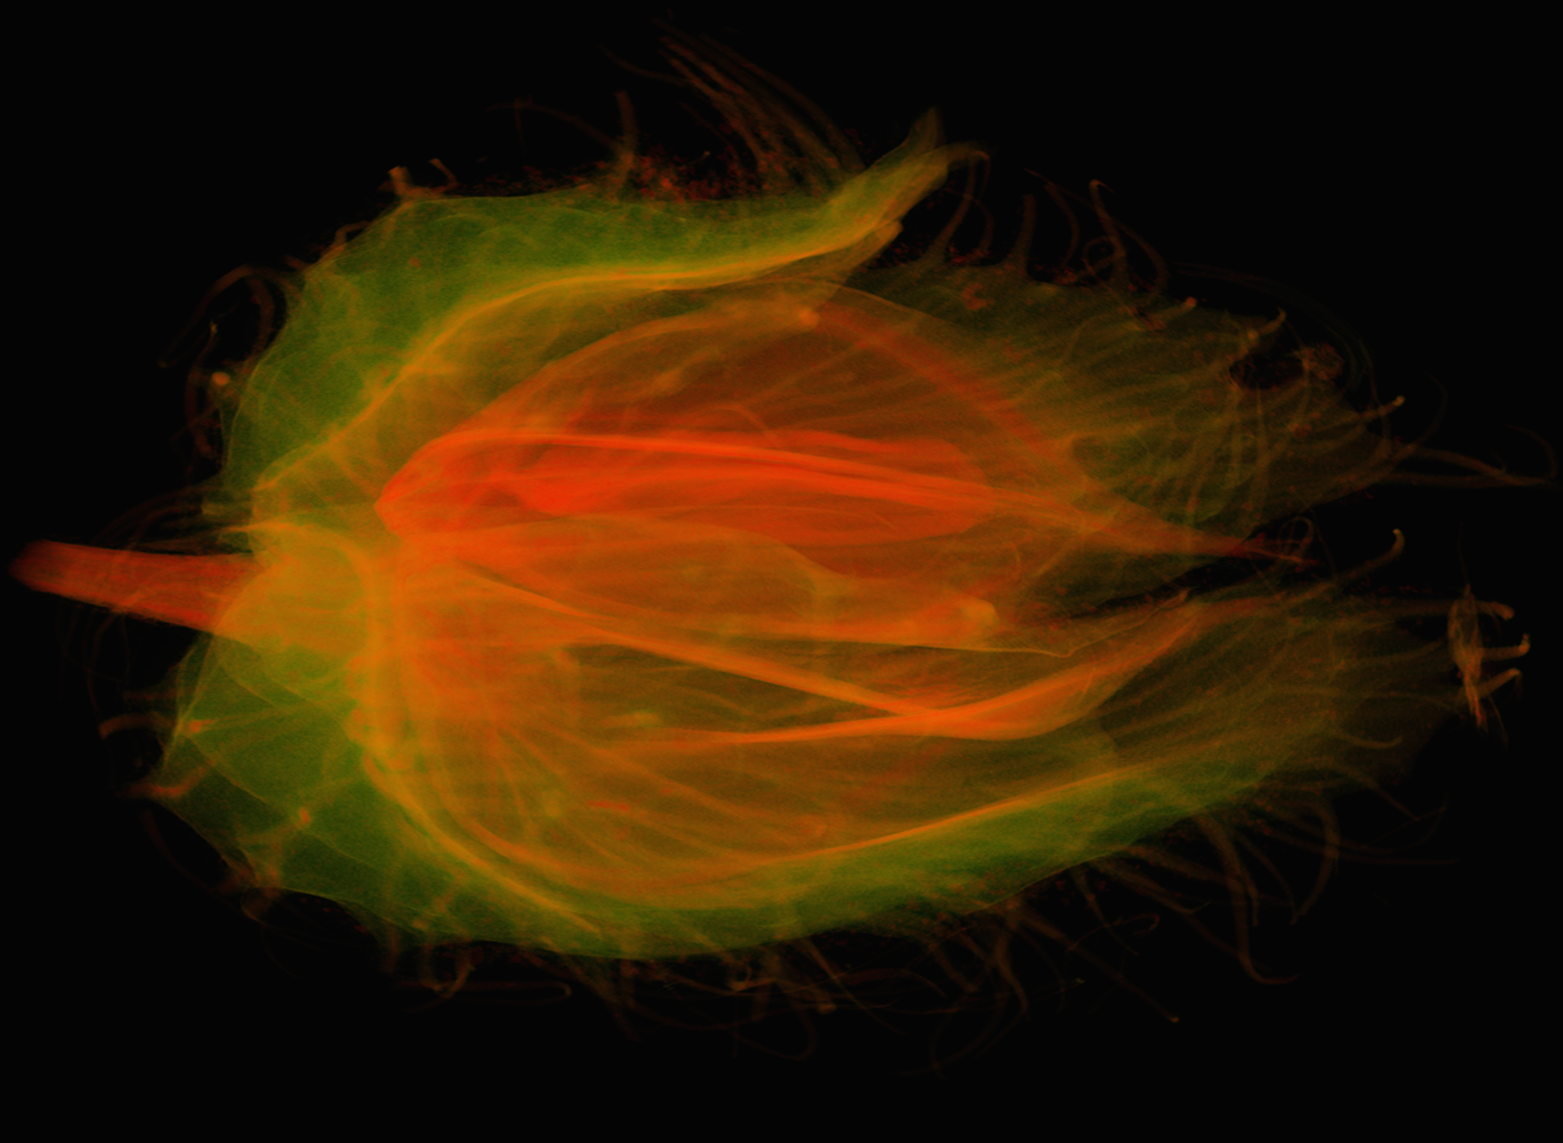
\includegraphics[height=.44\columnwidth]{images/beechnut}
  \caption{\label{fVolumes}Volumes used for object distribution benchmarks:
    spike frequencies of a three million neuron electrical simulation at
    512x437x240 unsigned byte (51MB, left) and an MicroCT scan of a beechnut at
    1024x1024x1546 unsigned short (3GB, right) resolution}
\end{figure}

The spike frequency volumes aggregate the number of spikes which happened within
a given voxel over a given time. The absolute spike count is renormalized to an
unsigned byte value during creation. Higher densities in the volume represent
higher spiking activity in the voxel.

\subsubsection{Data Compression Engines}

A critical piece for data distribution performance are the characteristics of
the data compression algorithm. Our microbenchmark compresses a set of binary
files, precalculating the speed and compression ratio of the various engines.
\fig{fCompressor} shows the compression and decompression speed in gigabyte per
second as well as the size of the compressed data relative to the uncompressed
data. The different ZSTD$x$ engines use the ZStandard compression library at
compression level $x$. The measurements were performed on a single, isolated
node.

\begin{figure}[ht]\center
  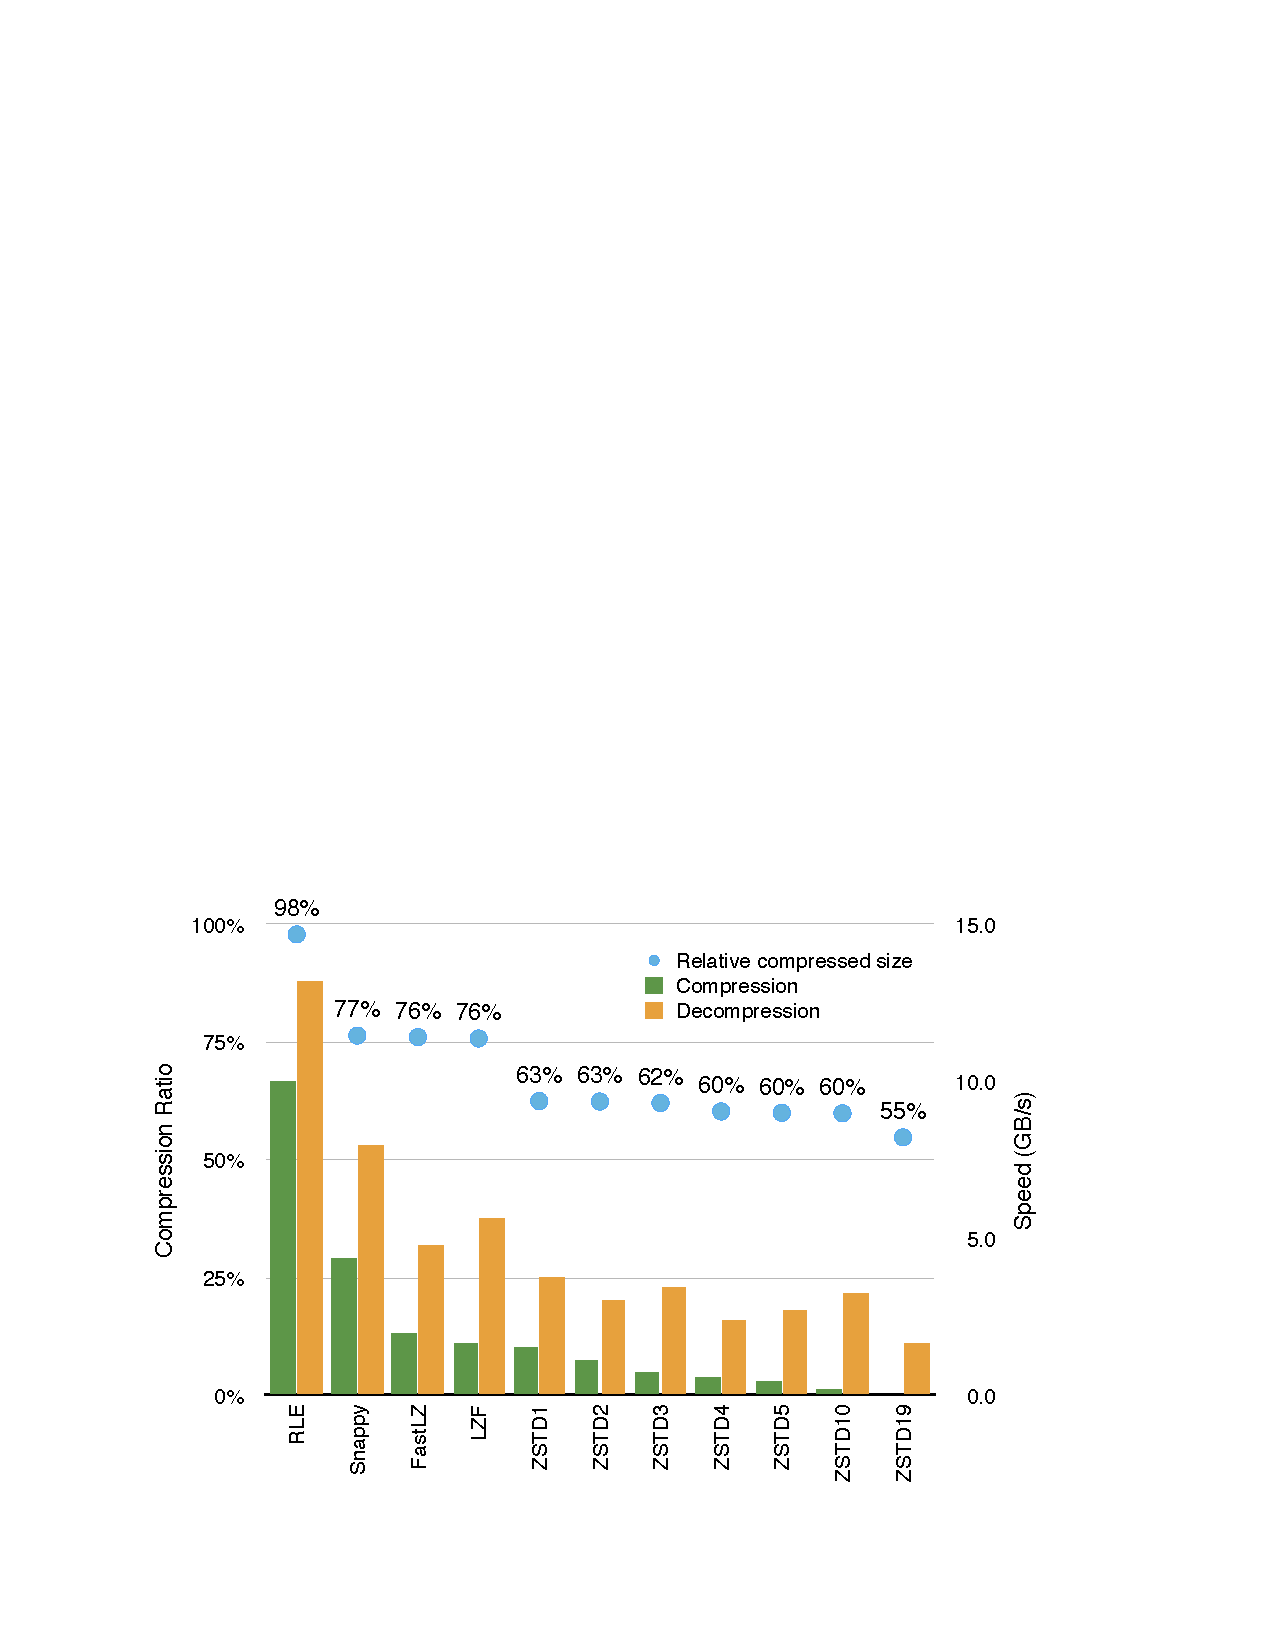
\includegraphics[width=\columnwidth]{images/compressor}
  \caption{\label{fCompressor}Data compression for generic binary data}
\end{figure}

RLE compression has a very low overhead but merely removes ``blank space'' in
the data. The Snappy compression, used as default in \textsf{Collage}, achieves
the same compression ratio as the LZ variants at a much higher speed. The
ZStandard compressor has roughly the same speed as the LZ variants at the lowest
compression level, but provides significantly better compression. At higher
compression levels it can improve the compression ratio slightly, but at a high
cost for the compression speed.

The compression ratio for the models used in the following section deviate from
this averaged distribution. \fig{fCompressorDetail} shows the compression ratios
for the triangle and volume data.

The ply data is little compressible, the default compressor achieves a 10\%
reduction. This is due to a high entropy in the data and the dominant use of
floating point values. Overall, the profile is similar to the generic benchmark,
at a smaller compression rate.

The volume data on the other hand is sparsely populated and using integer (byte
and short) values, which is easier to compress. The naive RLE implementation
already achieves a good compression rate, showing that the smaller volume contains at
most 28\% empty space and the bigger volume at most 43\%. Snappy and ZStandard
can reduce the spike data much further, reducing the data to a few megabytes.
Surprisingly, the beechnut data set does not yield significantly higher
compression with the modern Snappy and ZStandard libraries.


\subsubsection{Model Distribution and Update}

In this section we analyse how data distribution and synchronization performs in
real-world applications. We extracted the existing data distribution code from a
mesh renderer (eqPly) and a volume renderer (Livre) into a benchmark application
to measure the time to initially map all the objects on the render client nodes,
and to perform a commit-sync of the full data set after mapping has been
established. All figures observe a noticable measurement jitter due to other
services running on the cluster. The details of the benchmark algorithm can be
found in the
implementation\footnote{\htmladdnormallink{https://github.com/Eyescale/Equalizer/tree/paper2018/tools/eqObjectBench}}.
used the same data sets as in the previous section. We ran the benchmark on up
to eight physical nodes, that is, after eight processes nodes start to run two
processes per node, which share CPU, memory and network interface bandwidth.

Object mapping is measured using the following settings: \textbf{none}
distributes the raw, uncompressed, and unbuffered data, \textbf{compression}
uses the Snappy compressor to distribute unbuffered data, \textbf{buffered}
reuses uncompressed, serialized data for mappings from multiple nodes, and
\textbf{compression buffered} reused the compressed buffer for multiple nodes.
Unbuffered operations need to reserialize, and potentially recompress, the
master object data for each slave node. Each slave instance needs to deserialize
and decompress the data.

During data synchronization, the master instance commits the object data to all
mapped slave instances simultaneously. This is a ``push'' operation, whereas the
mapping is a slave-triggered ``pull'' operation with additional synchronization
points. Slave nodes queue this data and consume it during synchronization. We
test the time to commit and sync the data using different compression engines.


The David statue at 2mm resolution is organized in a kD-tree for rendering. Each
node is a separate distributed object, which has two child node objects. A
total of $1023$ objects is distributed and synchronized. \fig{fDavidDist} shows
the distribution times for this data set. Due to limited compressibility of the
data, the results are relatively similar. Compressing the data repeatedly for
each client leads to decreased performance, since the compression overhead
cannot be amortized by the decreased transmission time. Buffering data slightly
improves performance by reducing the CPU and copy overhead. Combining
compression and buffering leads to the best performance, although only by about
10\%.

During synchronization, data is pushed from the master process to all mapped
slaves using a unicast connection to each slave. While the results in the
\fig{fDavidDist} (middle) are relatively close to each other, we can still
observe how the tradeoff between compression ratio and speed influences overall
performance. Better, slower compression algorithms lead to improved overall
performance when amortized over many send operations.

The volume data sets are distributed in a single object, serializing the raw
volume buffer. The Spike volume data set has a significant compression ratio,
which is reflected by the results in \fig{fSpikesDist}. Compression for this
data is beneficial for transmitting data over a 10~Gb/s link even for a single
slave process only. Buffering has little benefit since the serialization of
volume data is trivial. Buffered compression makes a significant difference,
since the compression cost can be amortized over $n$ nodes, reaching raw data
transmission rates of 3.7 GB/s with the default Snappy compressor and at best
4.4 GB/s with ZStandard at level 1.

The distribution of the beechnut data set also behaves as expected
(\fig{fBeechnutDist}). Due to the larger object size, uncompressed transmission
is slightly faster compared to the Spike data set at 700 MB/s, and compressed
transmission does not improve the mapping performance, likely due to increased
memory pressure caused by the large data size. The comparison of the various
compression engines is consistent with the benchmarks in
\fig{fCompressorDetail}; RLE, Snappy and the LZ variants are very close to each
other, and ZSTD1 can provide better performance after four nodes due to the
better compression ratio.

Finally, we compare data distribution speed using different protocols. In this
benchmark, data synchronization time of the Spike volume data set is measured,
as in \fig{fSpikesDist} (middle). Buffering is enabled, and compression is
disabled to focus on the raw network performance. \fig{fIFDist} shows the
performance using various protocols.

Unsurprisingly, TCP over the faster InfiniBand link outperforms the cheaper ten
gigabit ethernet link by more than a factor of two. Unexpectedly, the native
RDMA connection performs worse, even though it outperforms IPoIB in a simple
peer-to-peer connection benchmark. This needs further investigation, but we
suspect the abstraction of a byte stream connection chosen by \textsf{Collage}
for historical reasons is not well suited for remote DMA semantics; that is,
one needs to design the network API around zero-copy semantics with managed
memory for modern high-speed transports. Both Infiniband connections show
significant measurement jitter.

Our RSP multicast implementation performs as expected. \textsf{Collage} starts
using multicast to commit new object versions when two or more clients are
mapped, since the transmission to a single client is better done using unicast.
RSP consistently outperforms unicast on the same physical interface and shows
good scaling behavior (2.5 times slower on 16 vs 2 clients on ethernet, 1.8
times slower on InfiniBand). The scaling is significantly better when only one
process per node is used (\fig{fIFDist}, middle: 30\% slower on ethernet,
nearly flat on InfiniBand). The increased transmission time with multiple
clients is caused by a higher probability of packet loss, which increases
significantly when using more than one process per node, as shown in
\fig{fIFDist}, right. This figure plots the number of retransmissions
divided by the number of datagrams. Infiniband outperforms ethernet slightly,
but is largely limited by the RSP implementation throughput of preparing and
queueing the datagrams to and from the protocol thread, which we observed in a
profiling analysis.

%----------------------------------------------------------------------
\section{Discussion and Conclusion}
%----------------------------------------------------------------------
\label{sec:conclusions}

We have presented a significantly improved generic parallel rendering system
over the original publication \cite{EMP:09}. While the original publication
motivated the system design, this publication describes a feature-rich, mature
implementation capable of supporting a wide variety of use cases. We doubled the
support for scalable rendering modes, many of which are presented here for the
first time. We present new runtime adaptations for better load balance and
performance, describe how common optimizations are integrated into the system,
making Equalizer the most generically available scalable rendering system.

Furthermore, we present many new features needed in parallel rendering
applications, from advanced Virtual Reality support to advanced display system
setup for 2D/3D integration, auto-configuration and runtime reconfiguration, and
an advanced network data synchronization library tailored to parallel rendering
applications. We highlight a few commercial and research applications
underlining the generic and versatile system implemenation.

With respect to the feature set implemented, we believe that Equalizer now
covers almost any scenario within its scope. For future work, we would like to
integrate new research for better scalability, new network implementations in
particular for modern zero-copy RDMA based transports, as well as extending the
Sequel abstraction layer for ease of use.

%----------------------------------------------------------------------
\appendices
% use section* for acknowledgment
\ifCLASSOPTIONcompsoc
  % The Computer Society usually uses the plural form
  \section*{Acknowledgments}
\else
  % regular IEEE prefers the singular form
  \section*{Acknowledgment}
\fi
%----------------------------------------------------------------------
We would like to thank and acknowledge the following institutions and projects
for providing the 3D geometry and volume test data sets: the Digital
Michelangelo Project, Stanford 3D Scanning Repository, Cyberware Inc.,
volvis.org and the Visual Human Project.
%
This work was partially supported by
the Swiss National Science Foundation Grants 200021-116329 and 200020-129525,
the Swiss Commission for Technology and Innovation CTI/KTI Project 9394.2 PFES-ES,
the EU FP7 People Programme (Marie Curie Actions) under REA Grant Agreement n$^{\circ}290227$ and
a Hasler Stiftung grant (project number $12097$).

We would also like to thank all supporters and contributors of
\textsf{Equalizer}, most notably RTT, the Blue Brain Project, the University of
Siegen, the Electronic Visualization Lab at the University of Illinois Chicago
and Dardo Kleiner.

% trigger a \newpage just before the given reference
% number - used to balance the columns on the last page
% adjust value as needed - may need to be readjusted if
% the document is modified later
%\IEEEtriggeratref{8}
% The "triggered" command can be changed if desired:
%\IEEEtriggercmd{\enlargethispage{-5in}}

% biography section
%
% If you have an EPS/PDF photo (graphicx package needed) extra braces are
% needed around the contents of the optional argument to biography to prevent
% the LaTeX parser from getting confused when it sees the complicated
% \includegraphics command within an optional argument. (You could create
% your own custom macro containing the \includegraphics command to make things
% simpler here.)

\begin{IEEEbiography}[{
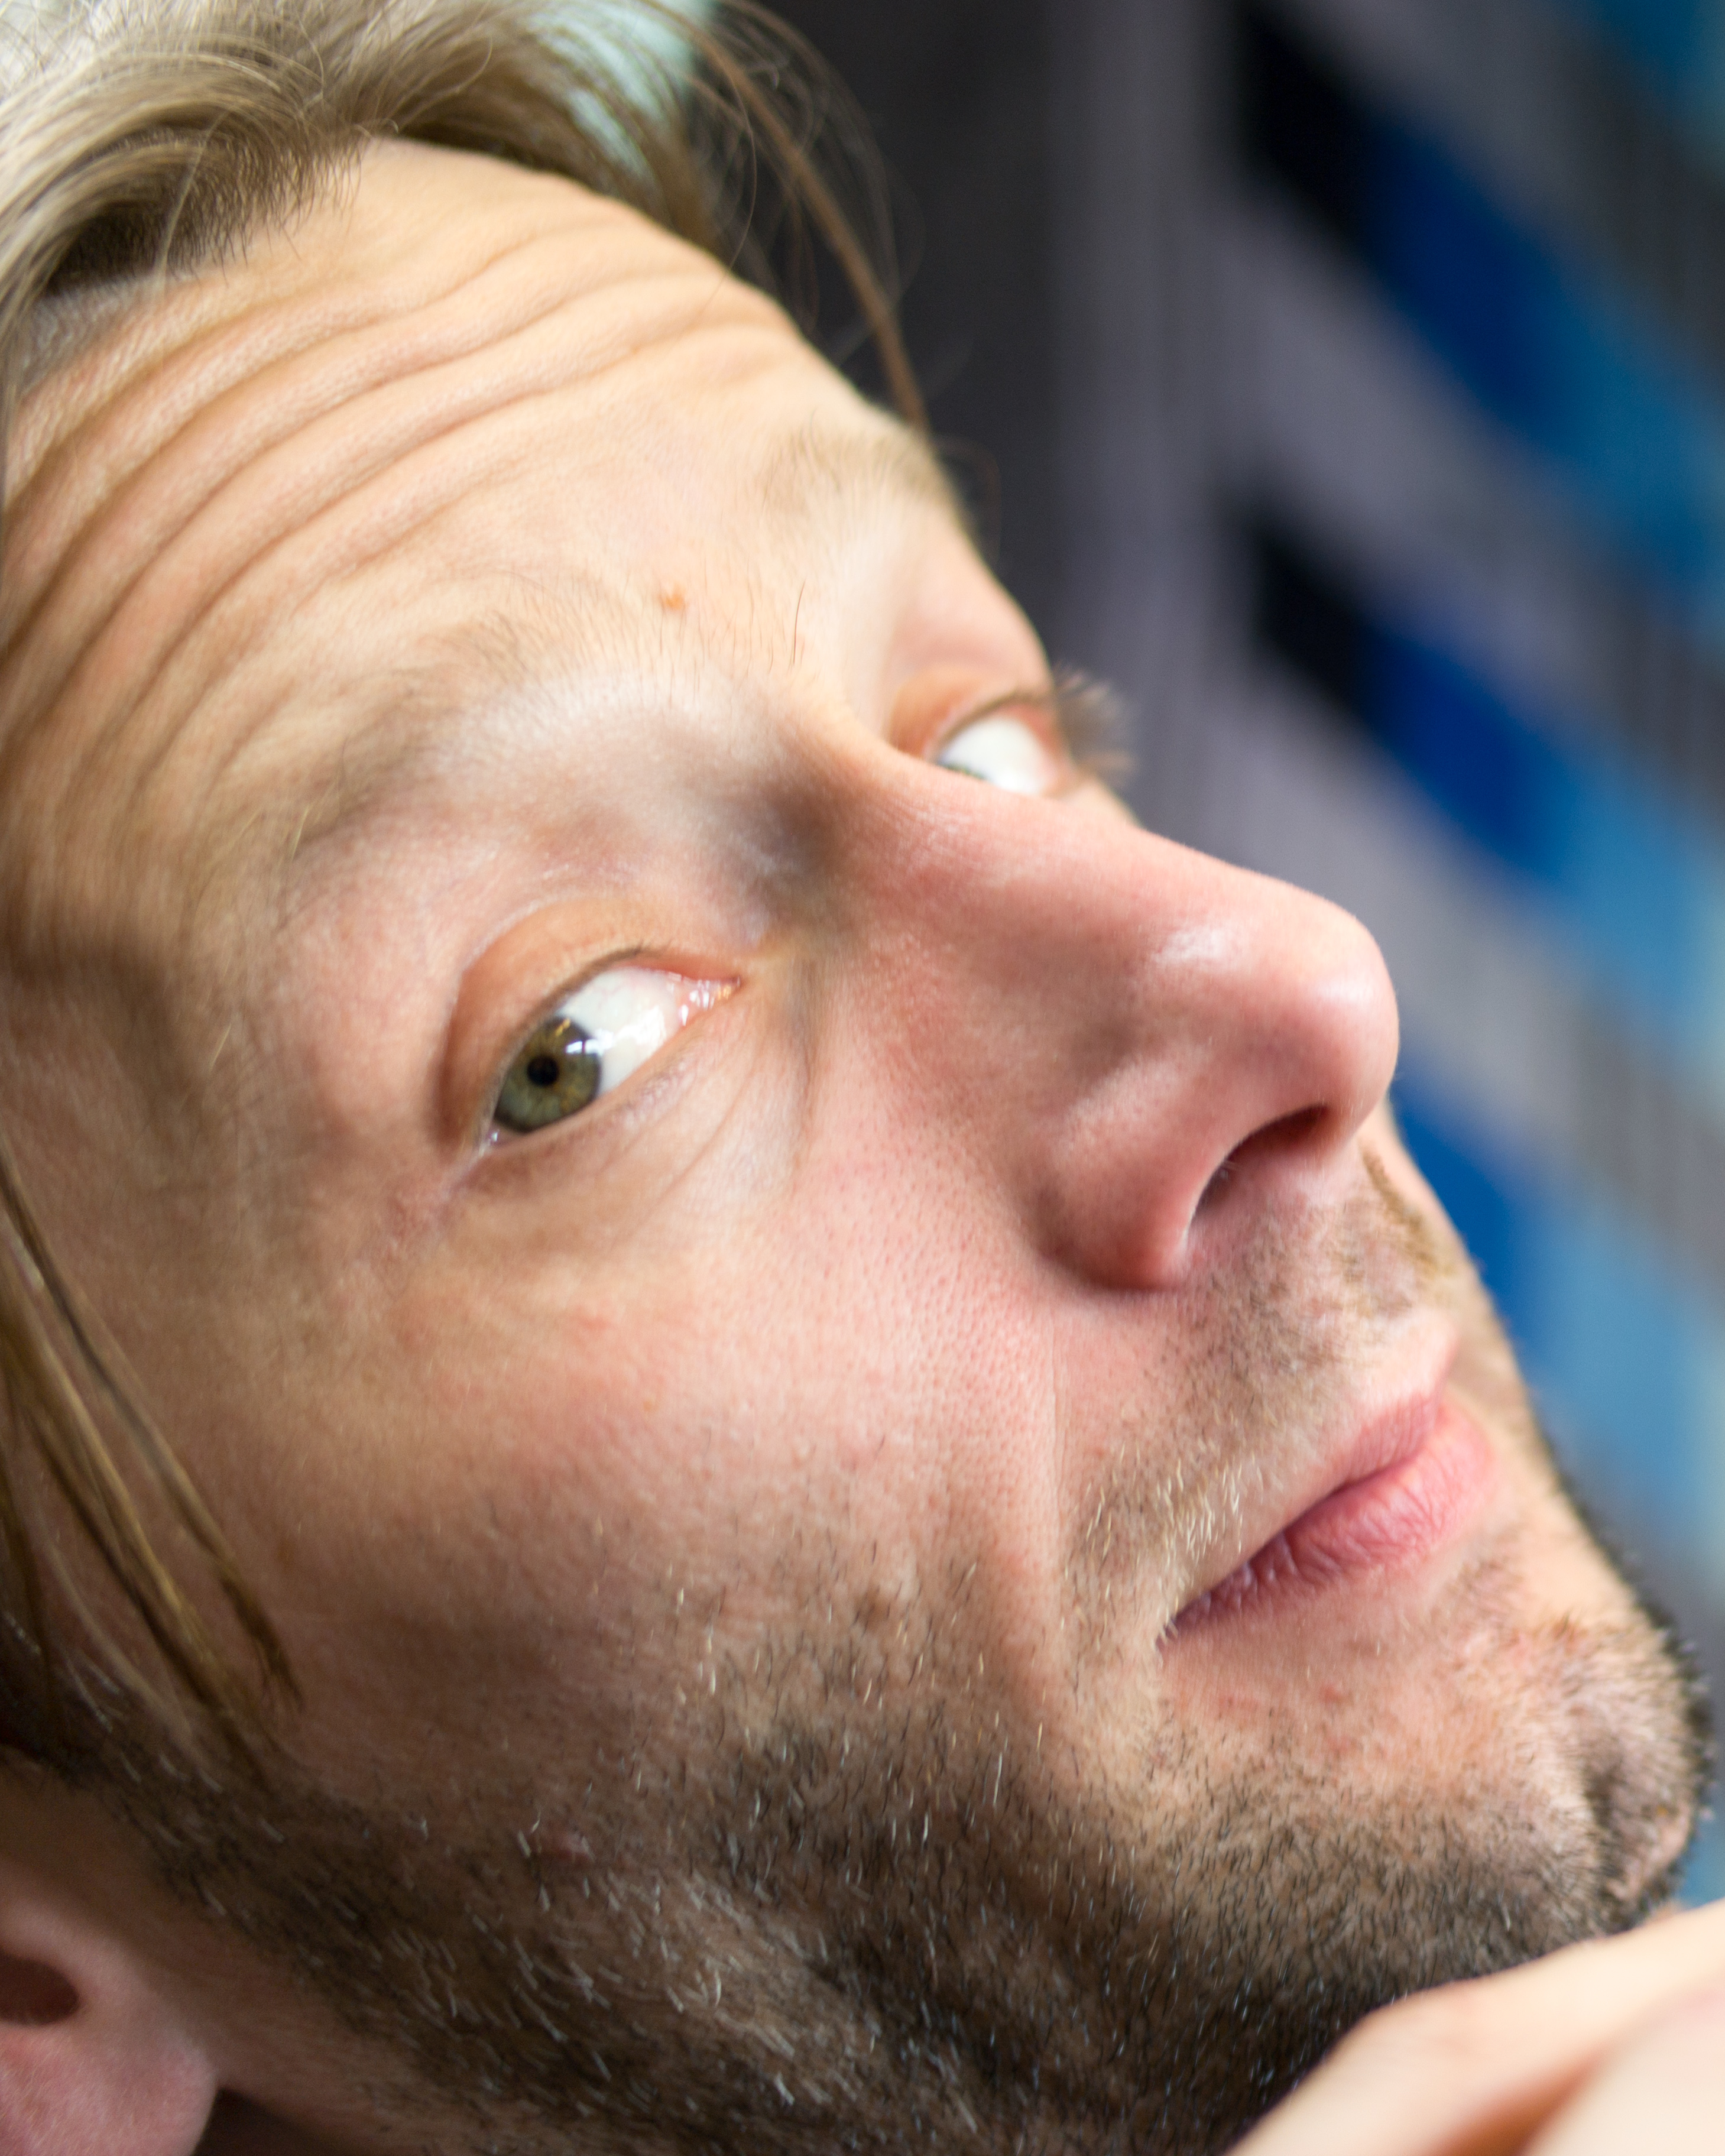
\includegraphics[width=1in,height=1.25in,clip,keepaspectratio]{images/stefan}}]{
Stefan Eilemann} Stefan is the technical manager of the Visualization Team in
the Blue
Brain Project. His work involves working towards large-scale visualization for
Exascale simulations; interactive integration of simulation, analysis and
visualization as well as flexible frameworks for data sharing and dynamic
allocation of heterogenous resources. He is the CEO and founder of Eyescale and
also the lead developer of the \textsf{Equalizer} parallel rendering framework.
He has worked in SGI's Advanced Graphics Division as the technical lead of
OpenGL Multipipe SDK - a toolkit for scalable, parallel visualization software
on shared memory supercomputers. He received his masters degree in Computer
Science from EPFL in 2015, and his Engineering Diploma in Computer Science in
1998. He is currently working towards a PhD in Computer Science at the
Visualization and MultiMedia Lab at the University of Zurich.
\end{IEEEbiography}

\begin{IEEEbiography}[{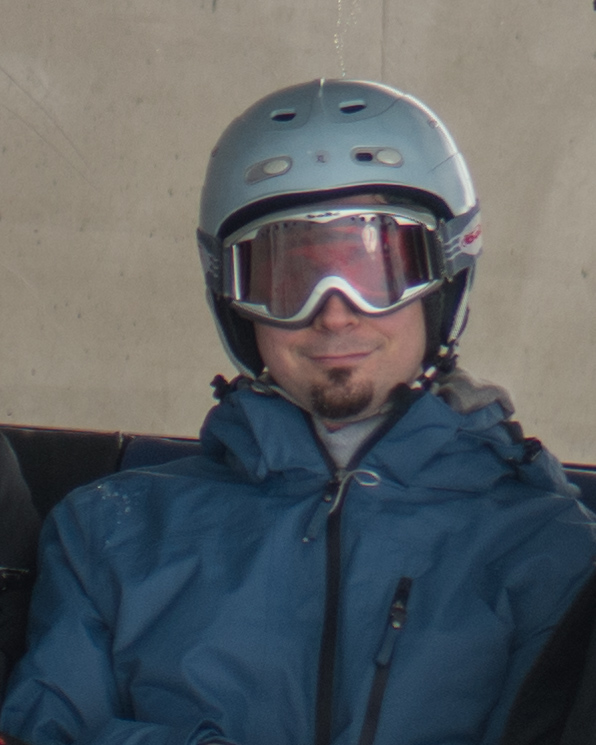
\includegraphics[width=1in,height=1.25in,clip,keepaspectratio]{images/david_steiner_picture2}}]{David Steiner}
received MSc degrees from the University of Applied Sciences Upper Austria (Digital Media) and the University of Zurich (Computer Science). He joined the Visualization and MultiMedia Lab (VMML) in 2012 and is currently pursuing his doctorate. His research interests include interactive large-scale data visualization, distributed parallel rendering, and load balancing.
\end{IEEEbiography}

\begin{IEEEbiography}[{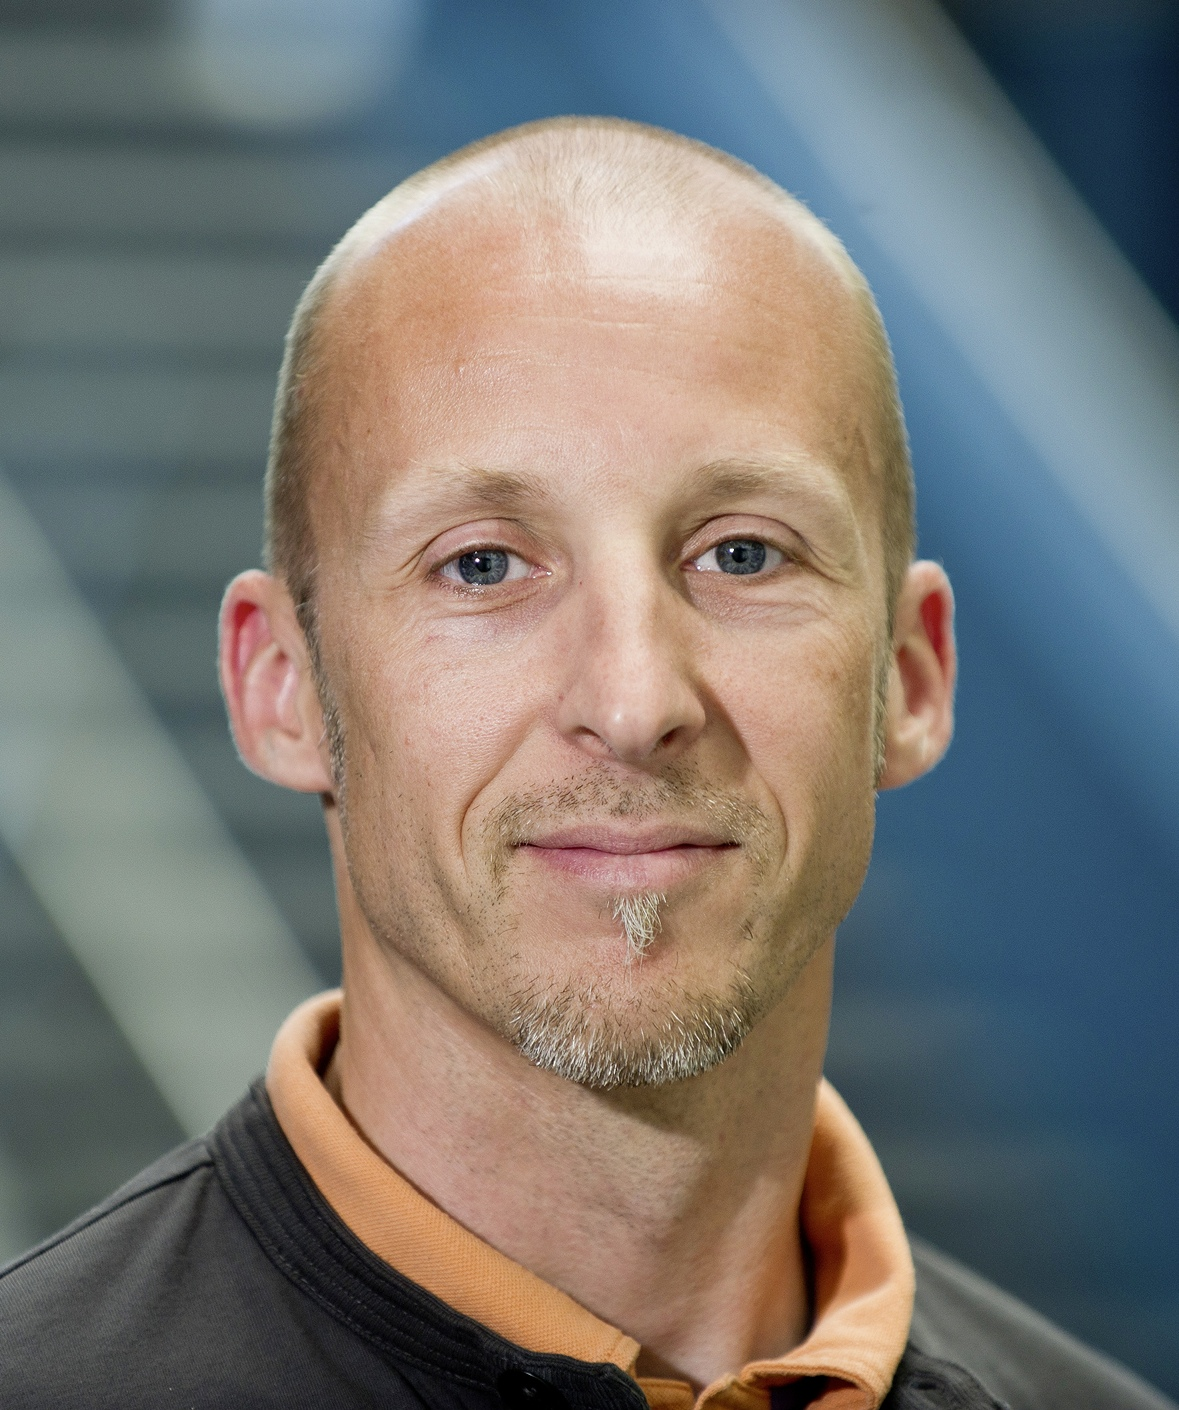
\includegraphics[width=1in,height=1.25in,clip,keepaspectratio]{images/renato}}]{Prof. Dr. Renato Pajarola}
has been a Professor in computer science at the University of Zurich since 2005, leading the Visualization and MultiMedia Lab (VMML). He has previously been an Assistant Professor at the University of California Irvine and a Postdoc at Georgia Tech. He has received his Dipl. Inf-Ing. ETH and Dr. sc. techn. degrees in computer science from the Swiss Federal Institute of Technology (ETH) Zurich in 1994 and 1998 respectively. He is a Fellow of the Eurographics Association and a Senior Member of both ACM and IEEE. His research interests include real-time 3D graphics, interactive data visualization and geometry processing.
\end{IEEEbiography}

% insert where needed to balance the two columns on the last page with
% biographies
% \newpage

\bibliographystyle{abbrv}
\bibliography{references}

\begin{figure*}[ht]\center
  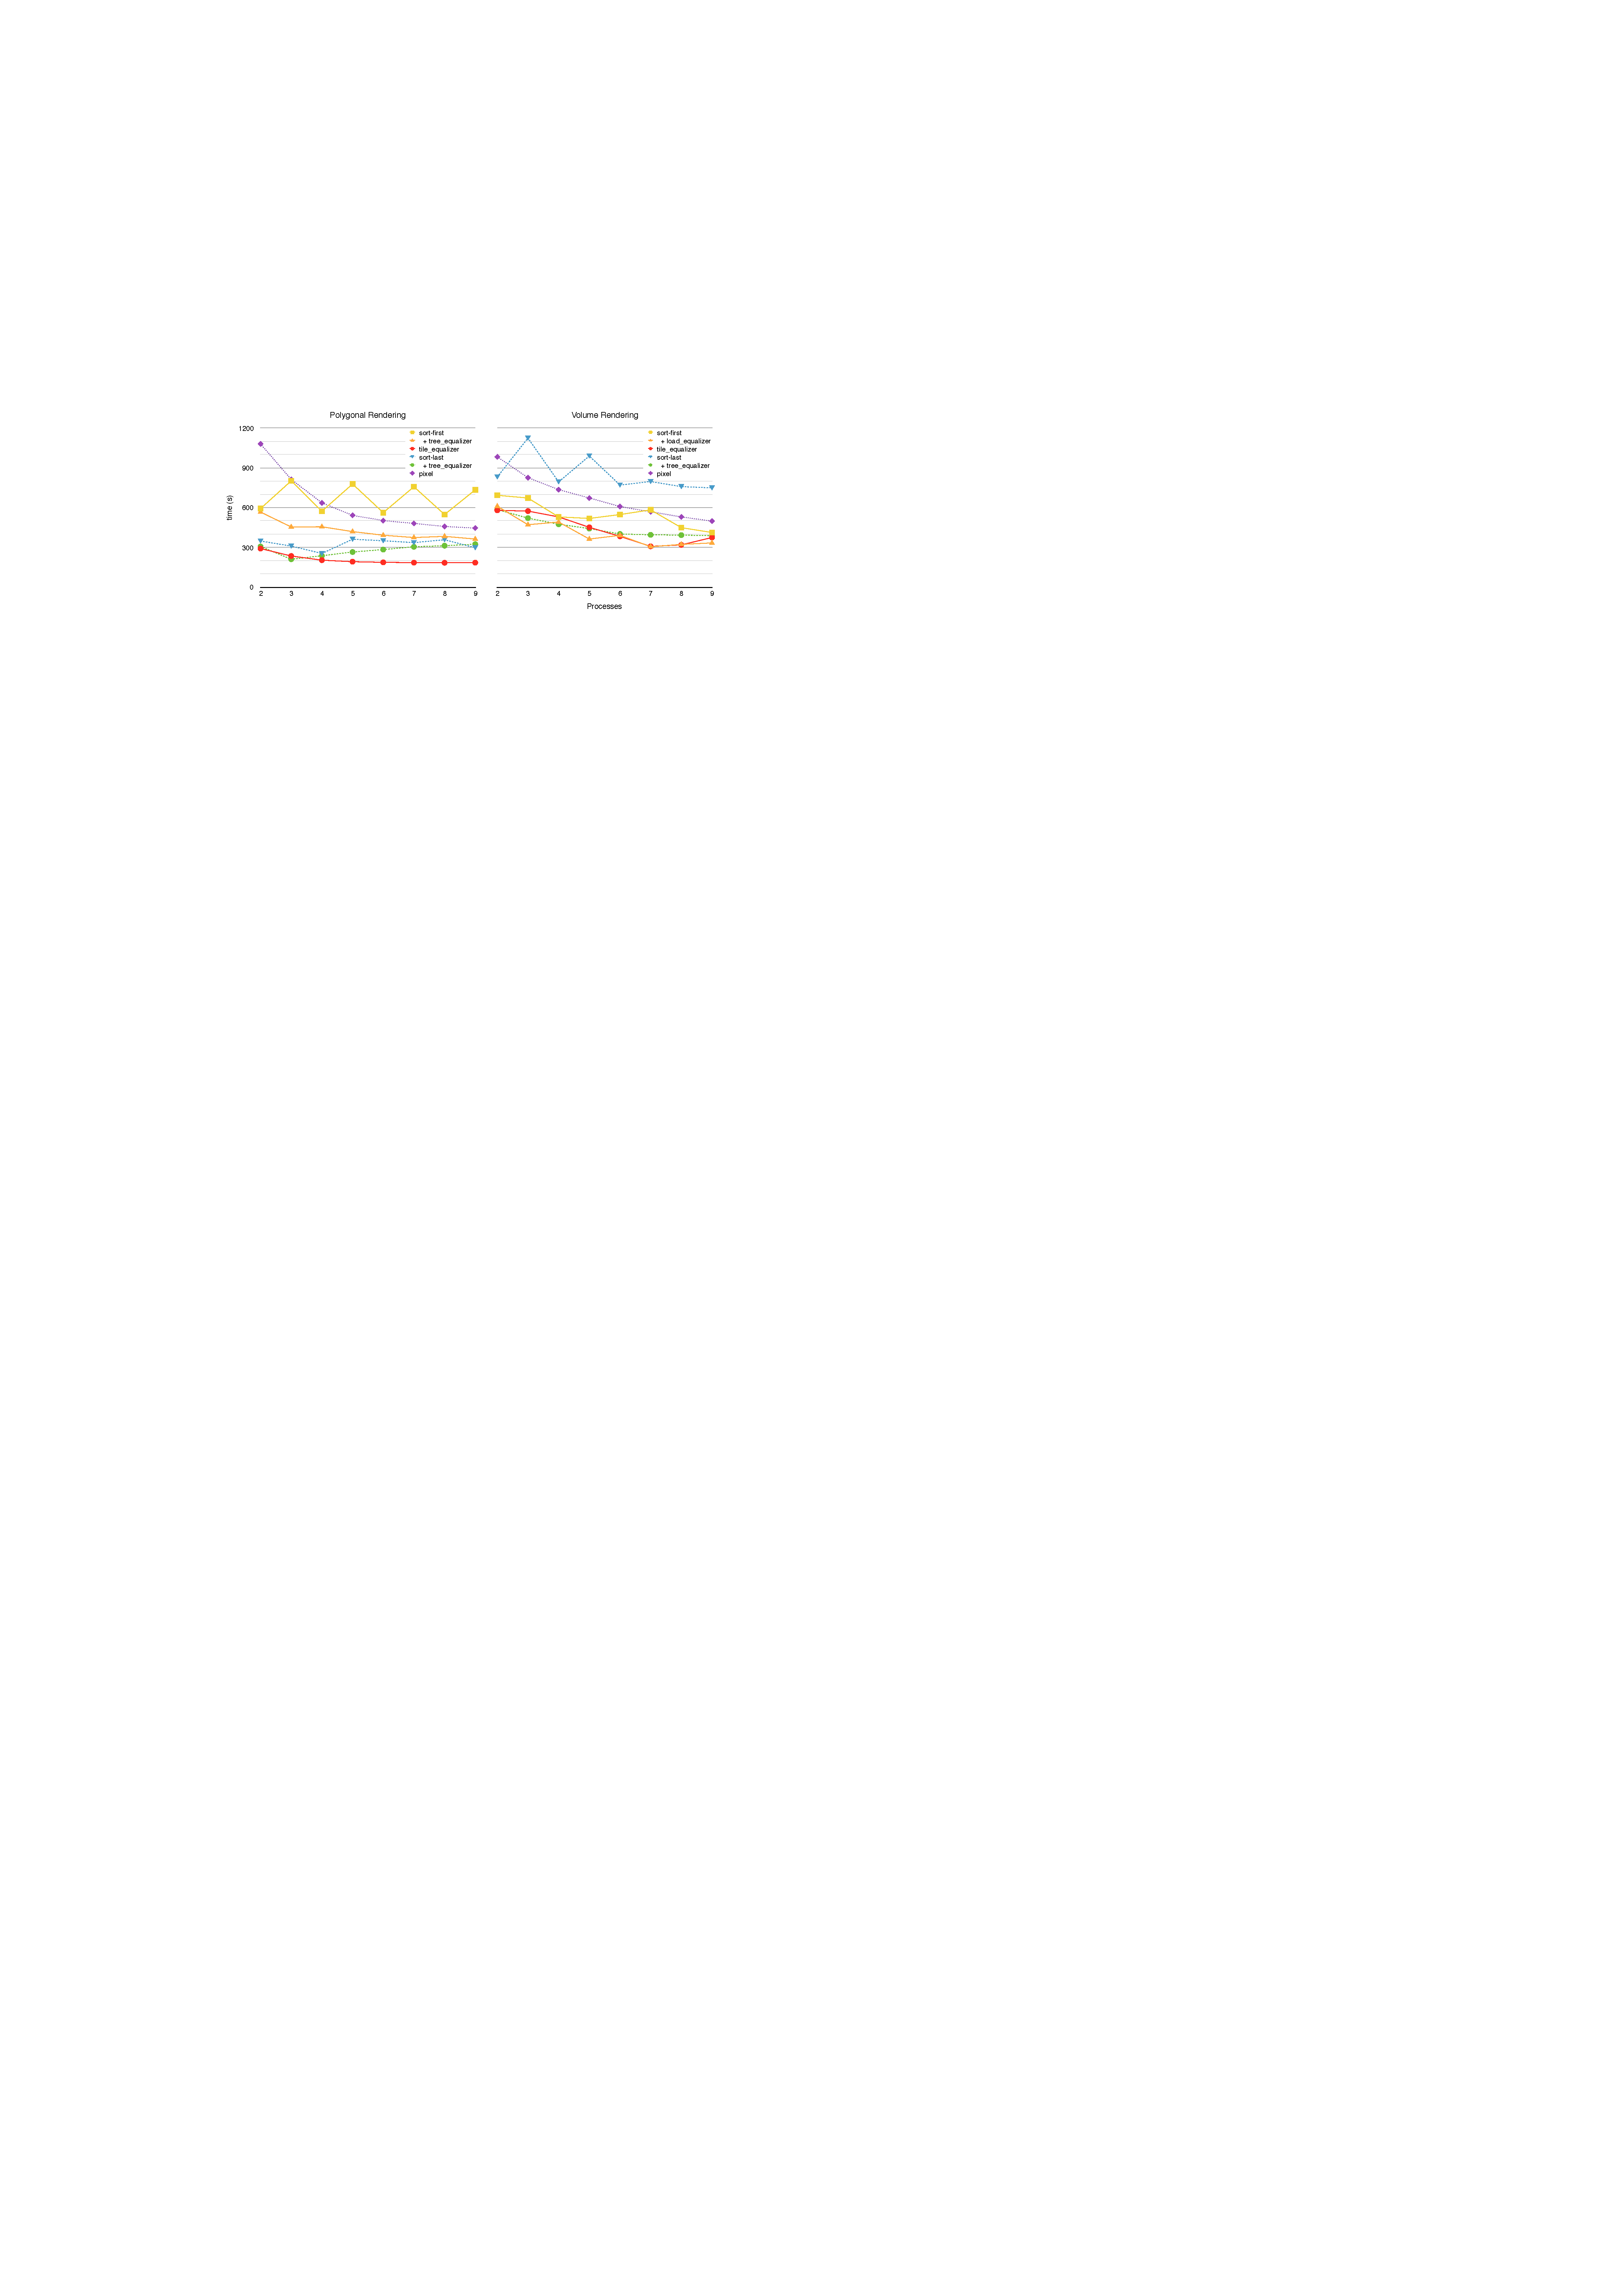
\includegraphics[width=\textwidth]{images/compounds}
  \caption{\label{fCompounds}Compound scalability for polygonal and volume data}
\end{figure*}

\begin{figure*}[ht]\center
  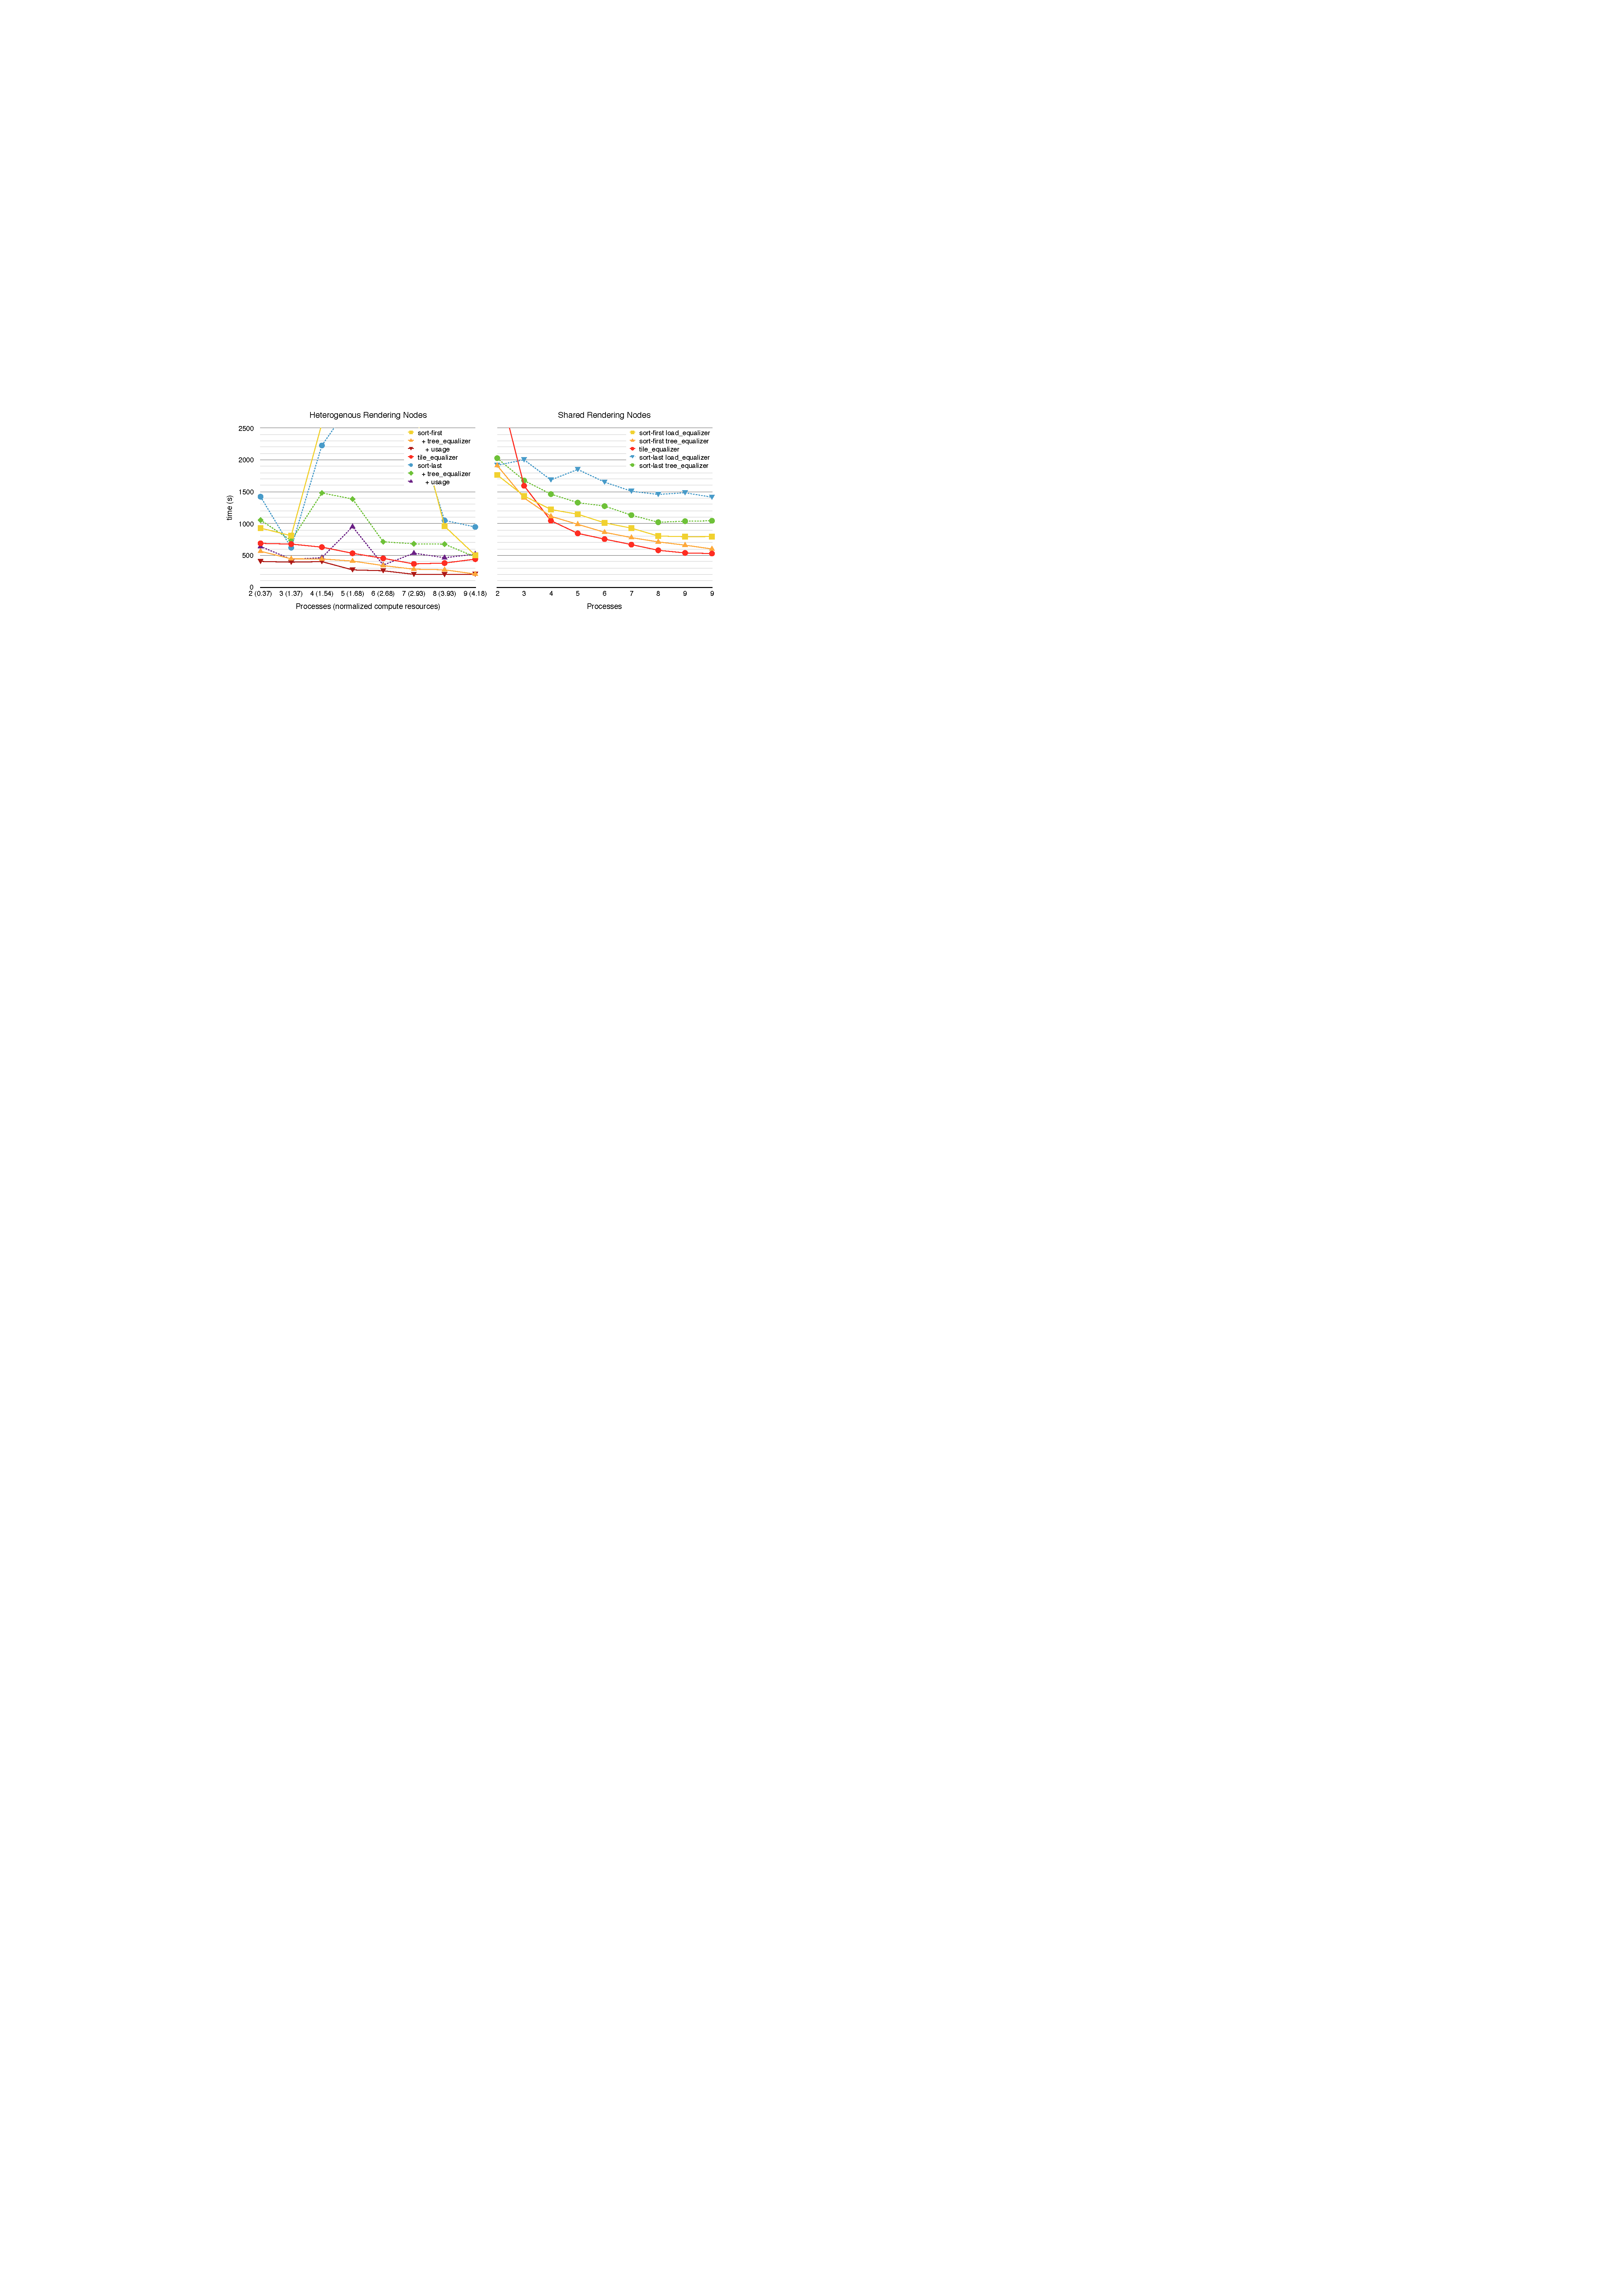
\includegraphics[width=\textwidth]{images/equalizers}
  \caption{\label{fEqualizers}Scalability with heterogenous rendering resources}
\end{figure*}

\begin{figure*}[ht]\center
  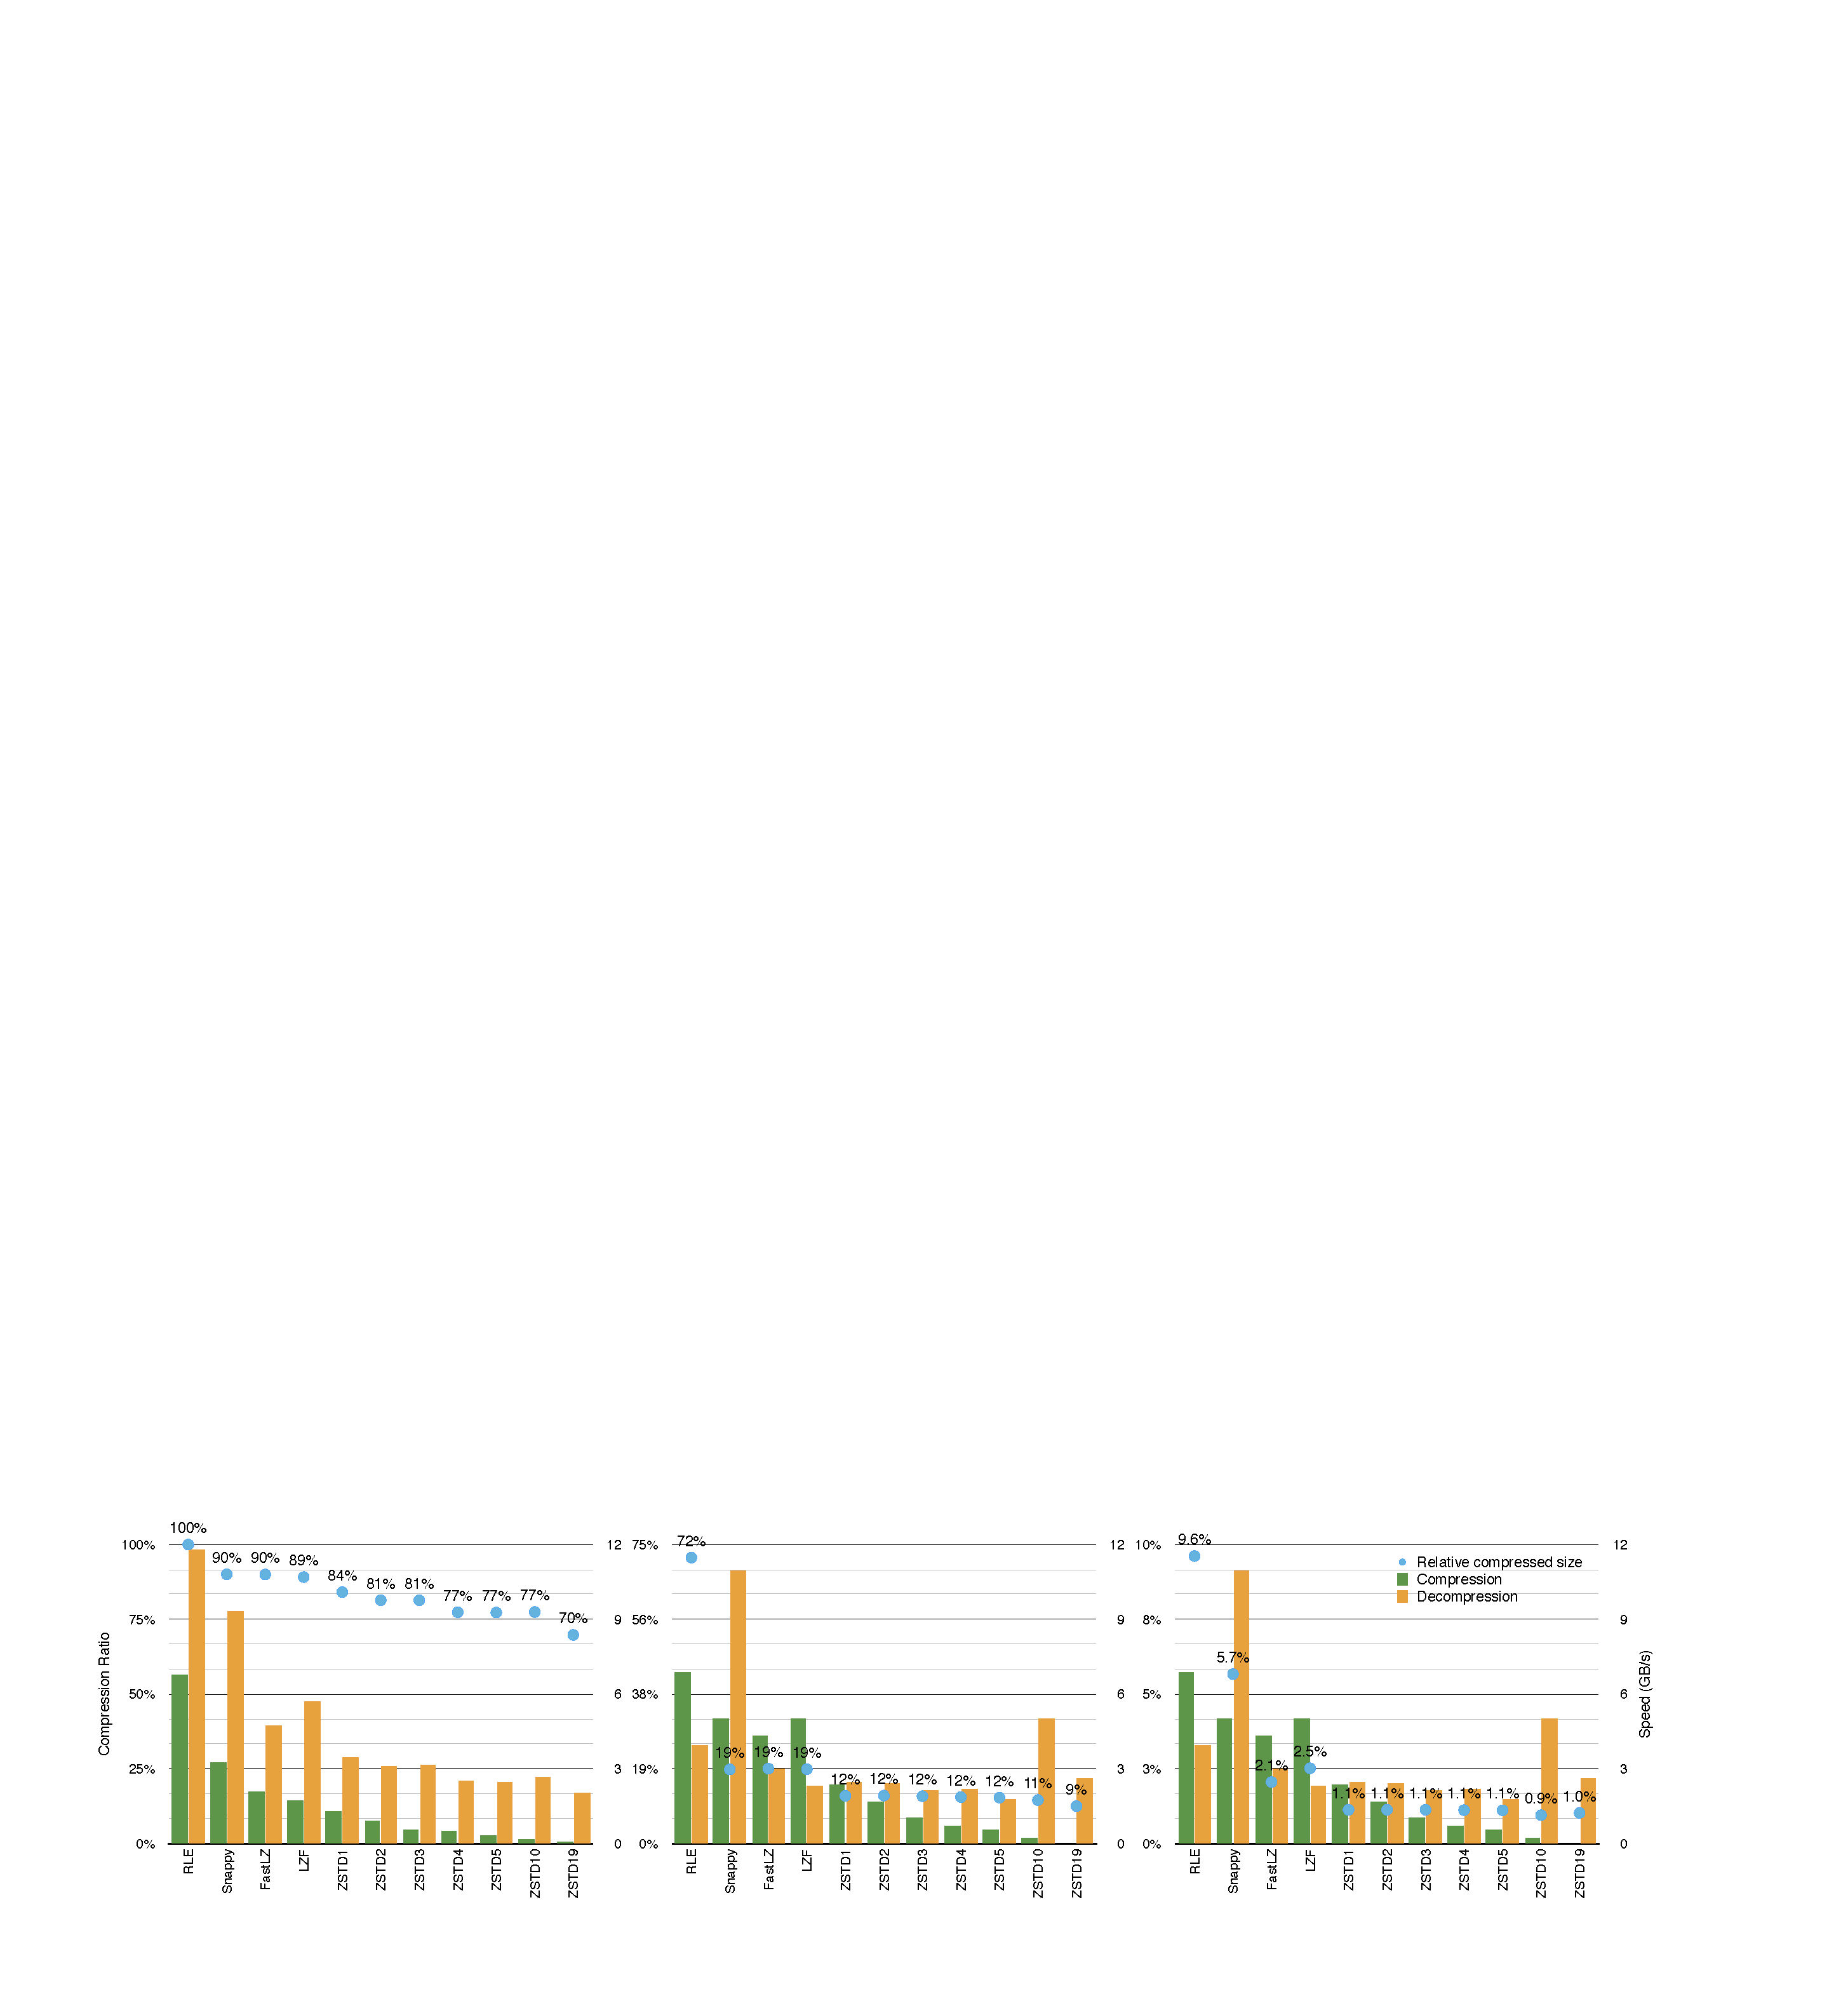
\includegraphics[width=\textwidth]{images/compressorDetail}
  \caption{\label{fCompressorDetail}Data compression for ply data (left, David
    statue 2mm) and raw volumes shown in \fig{fVolumes} (middle and right)}
\end{figure*}

\begin{figure*}[p!]\center
  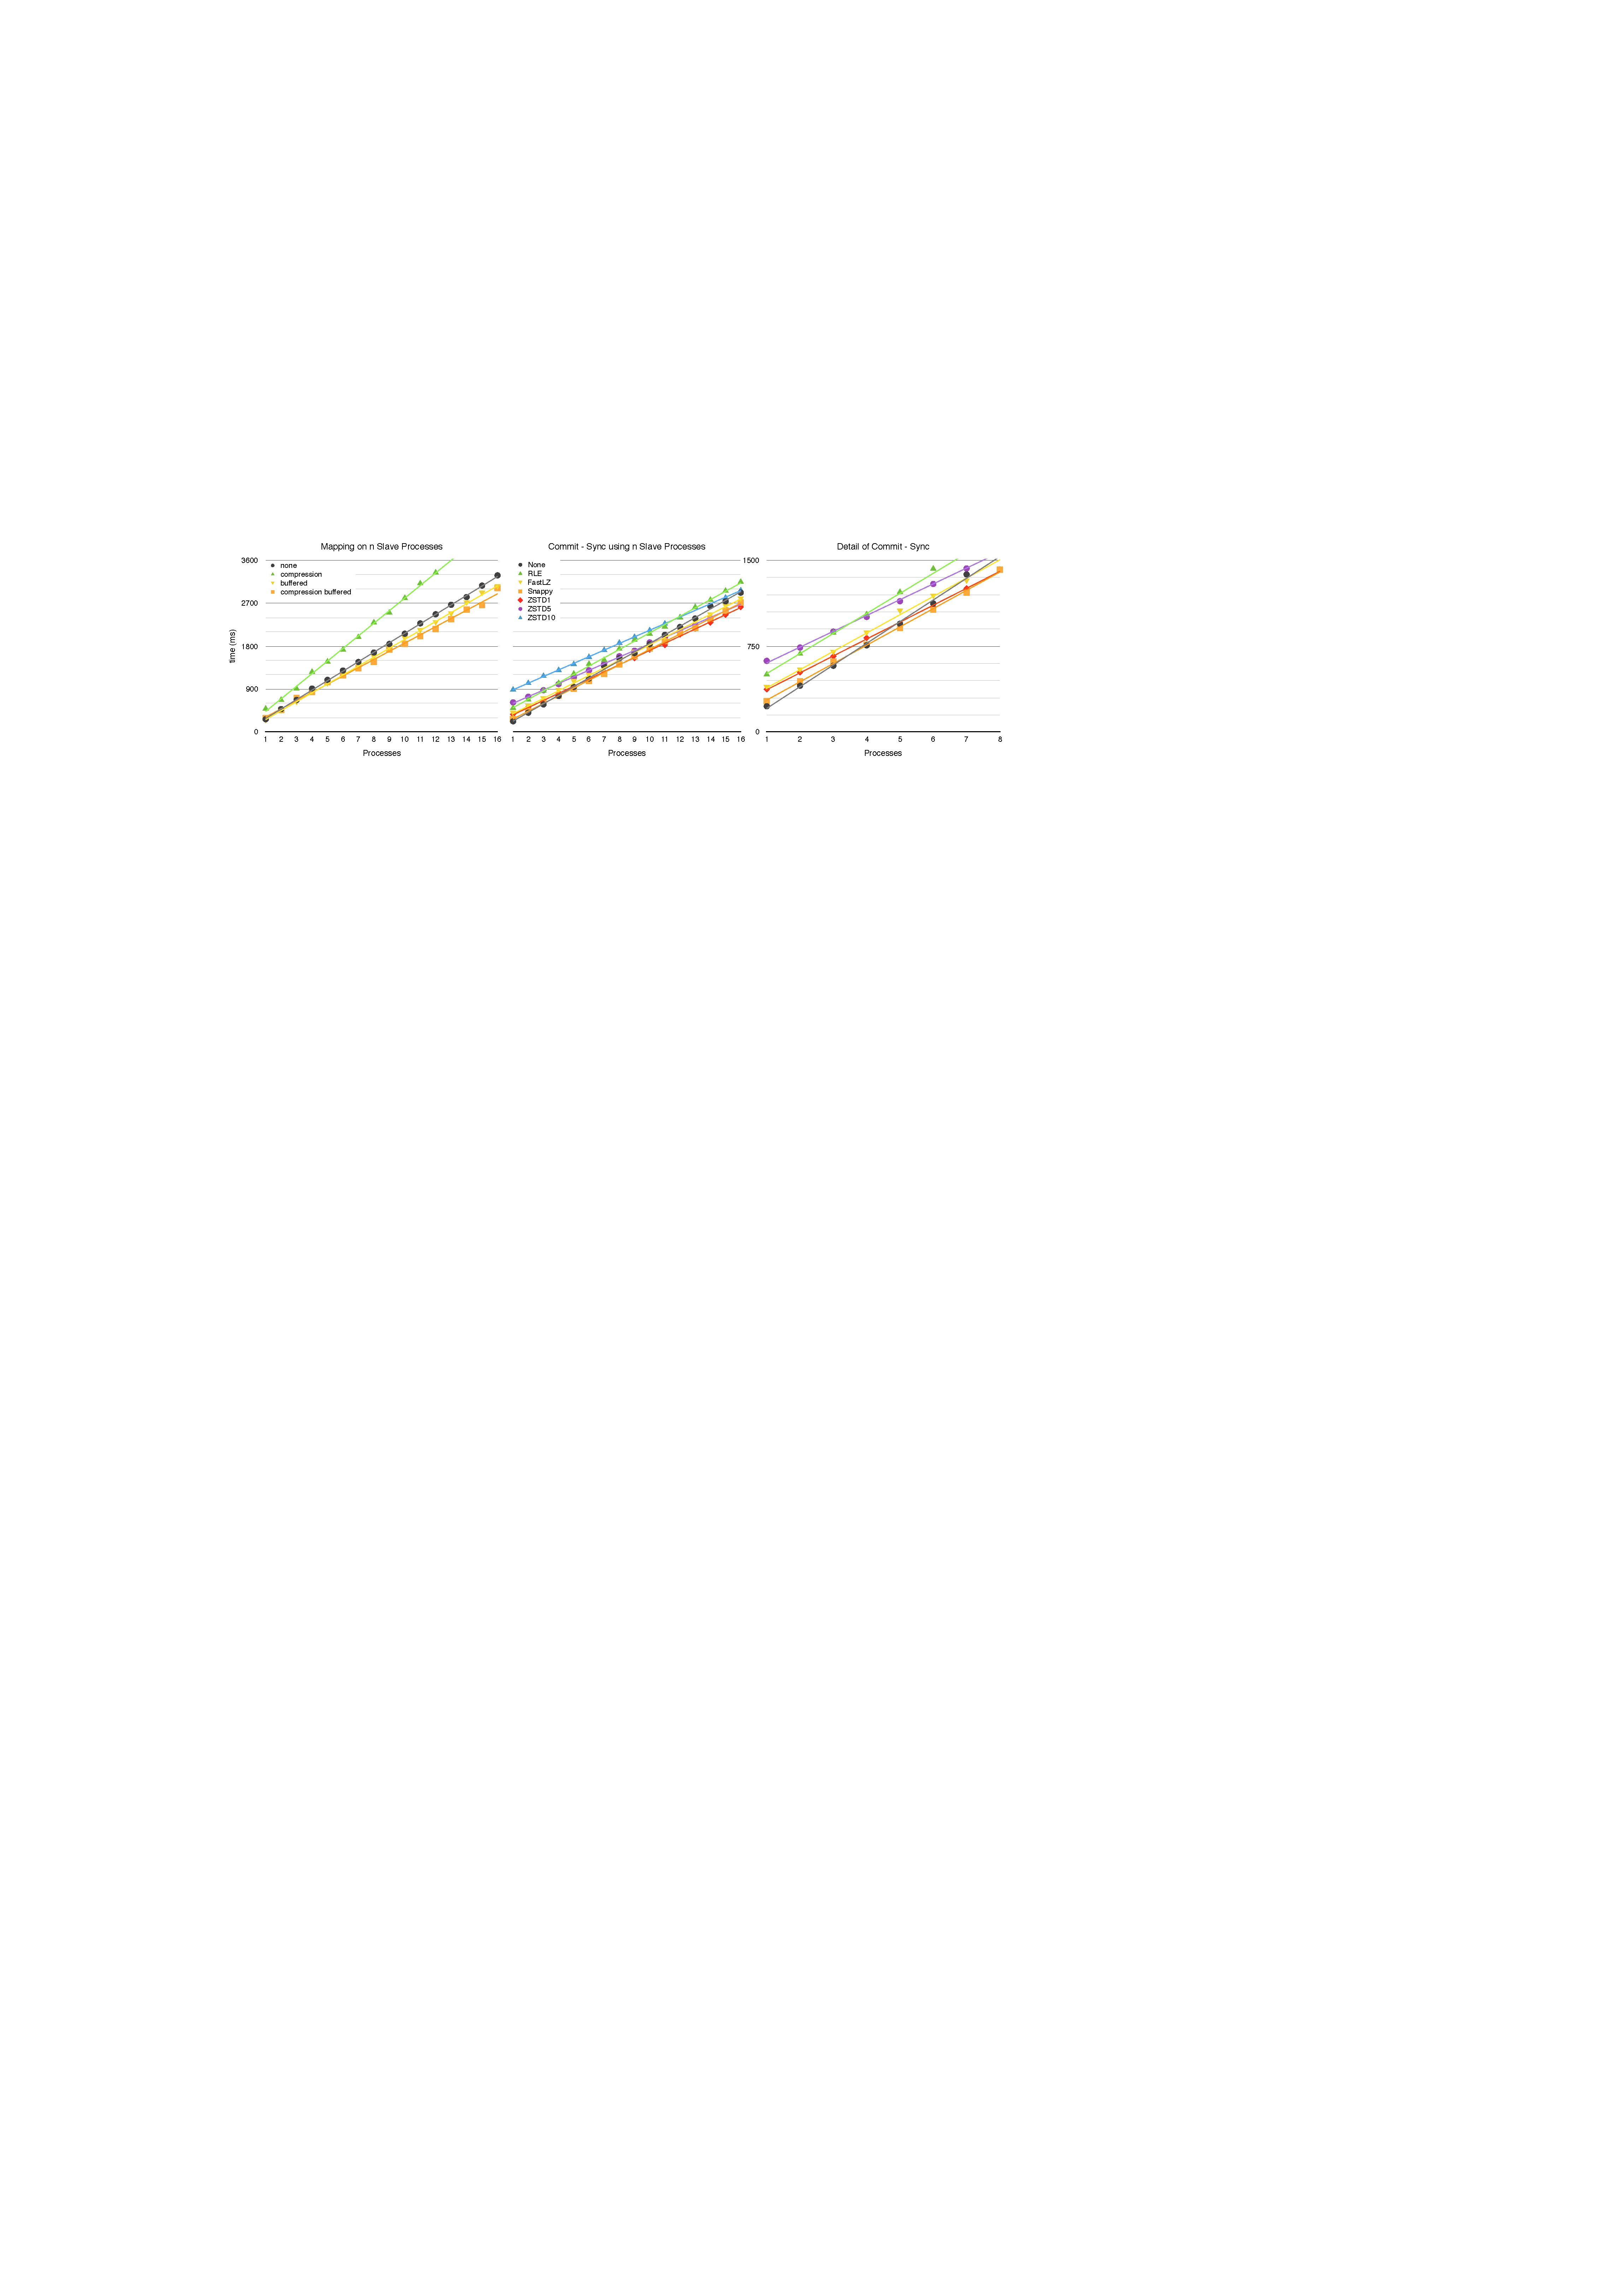
\includegraphics[height=.19\textheight]{images/daviddist}
  \caption{\label{fDavidDist}Object mapping (left) and data synchronization
    time (middle, detail view right) for the David 2mm data set in
    \fig{fDavid2mm}}
\end{figure*}
\begin{figure*}[p!]\center
  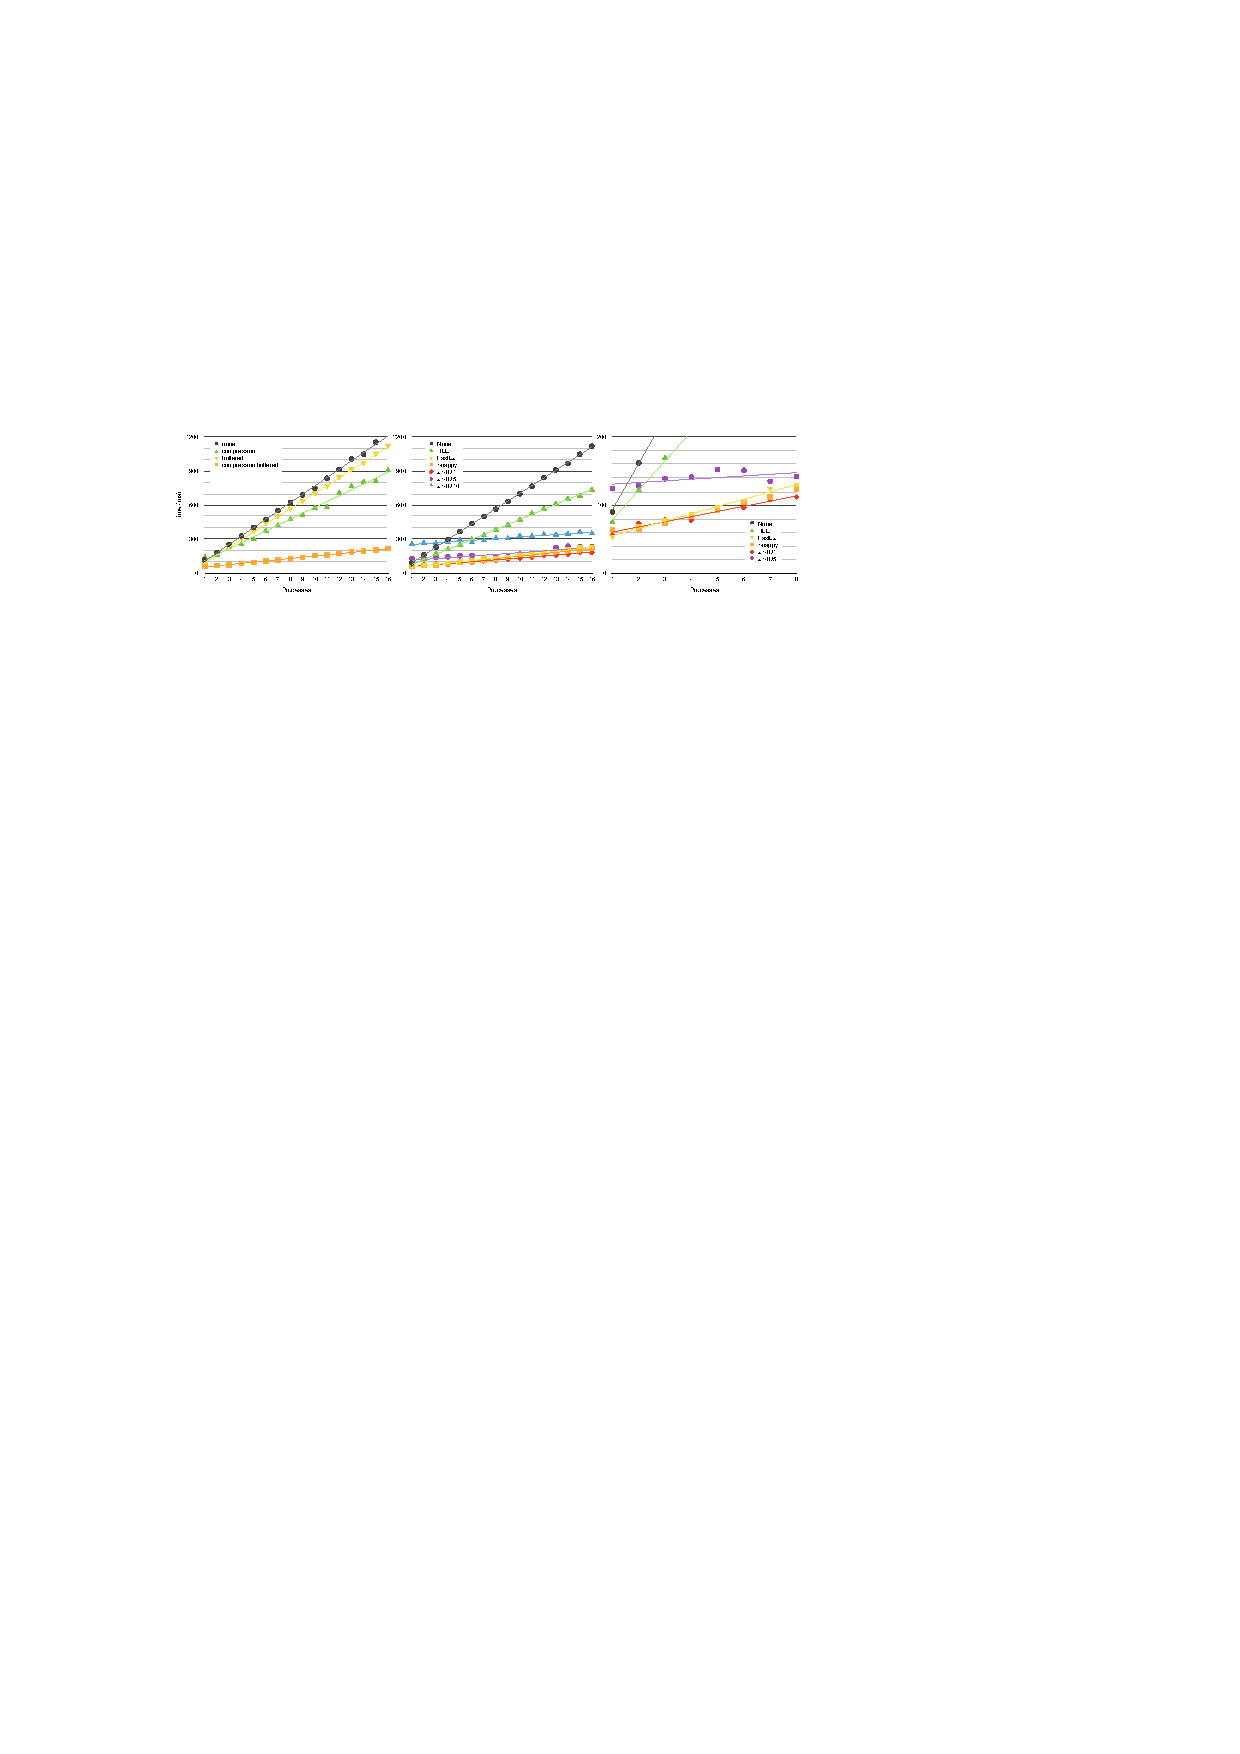
\includegraphics[height=.19\textheight]{images/spikesdist}
  \caption{\label{fSpikesDist}Object mapping (left) and data synchronization
    time (middle, detail view right) for the Spike data set in
    \fig{fVolumes}, left}
\end{figure*}
\begin{figure*}[p!]\center
  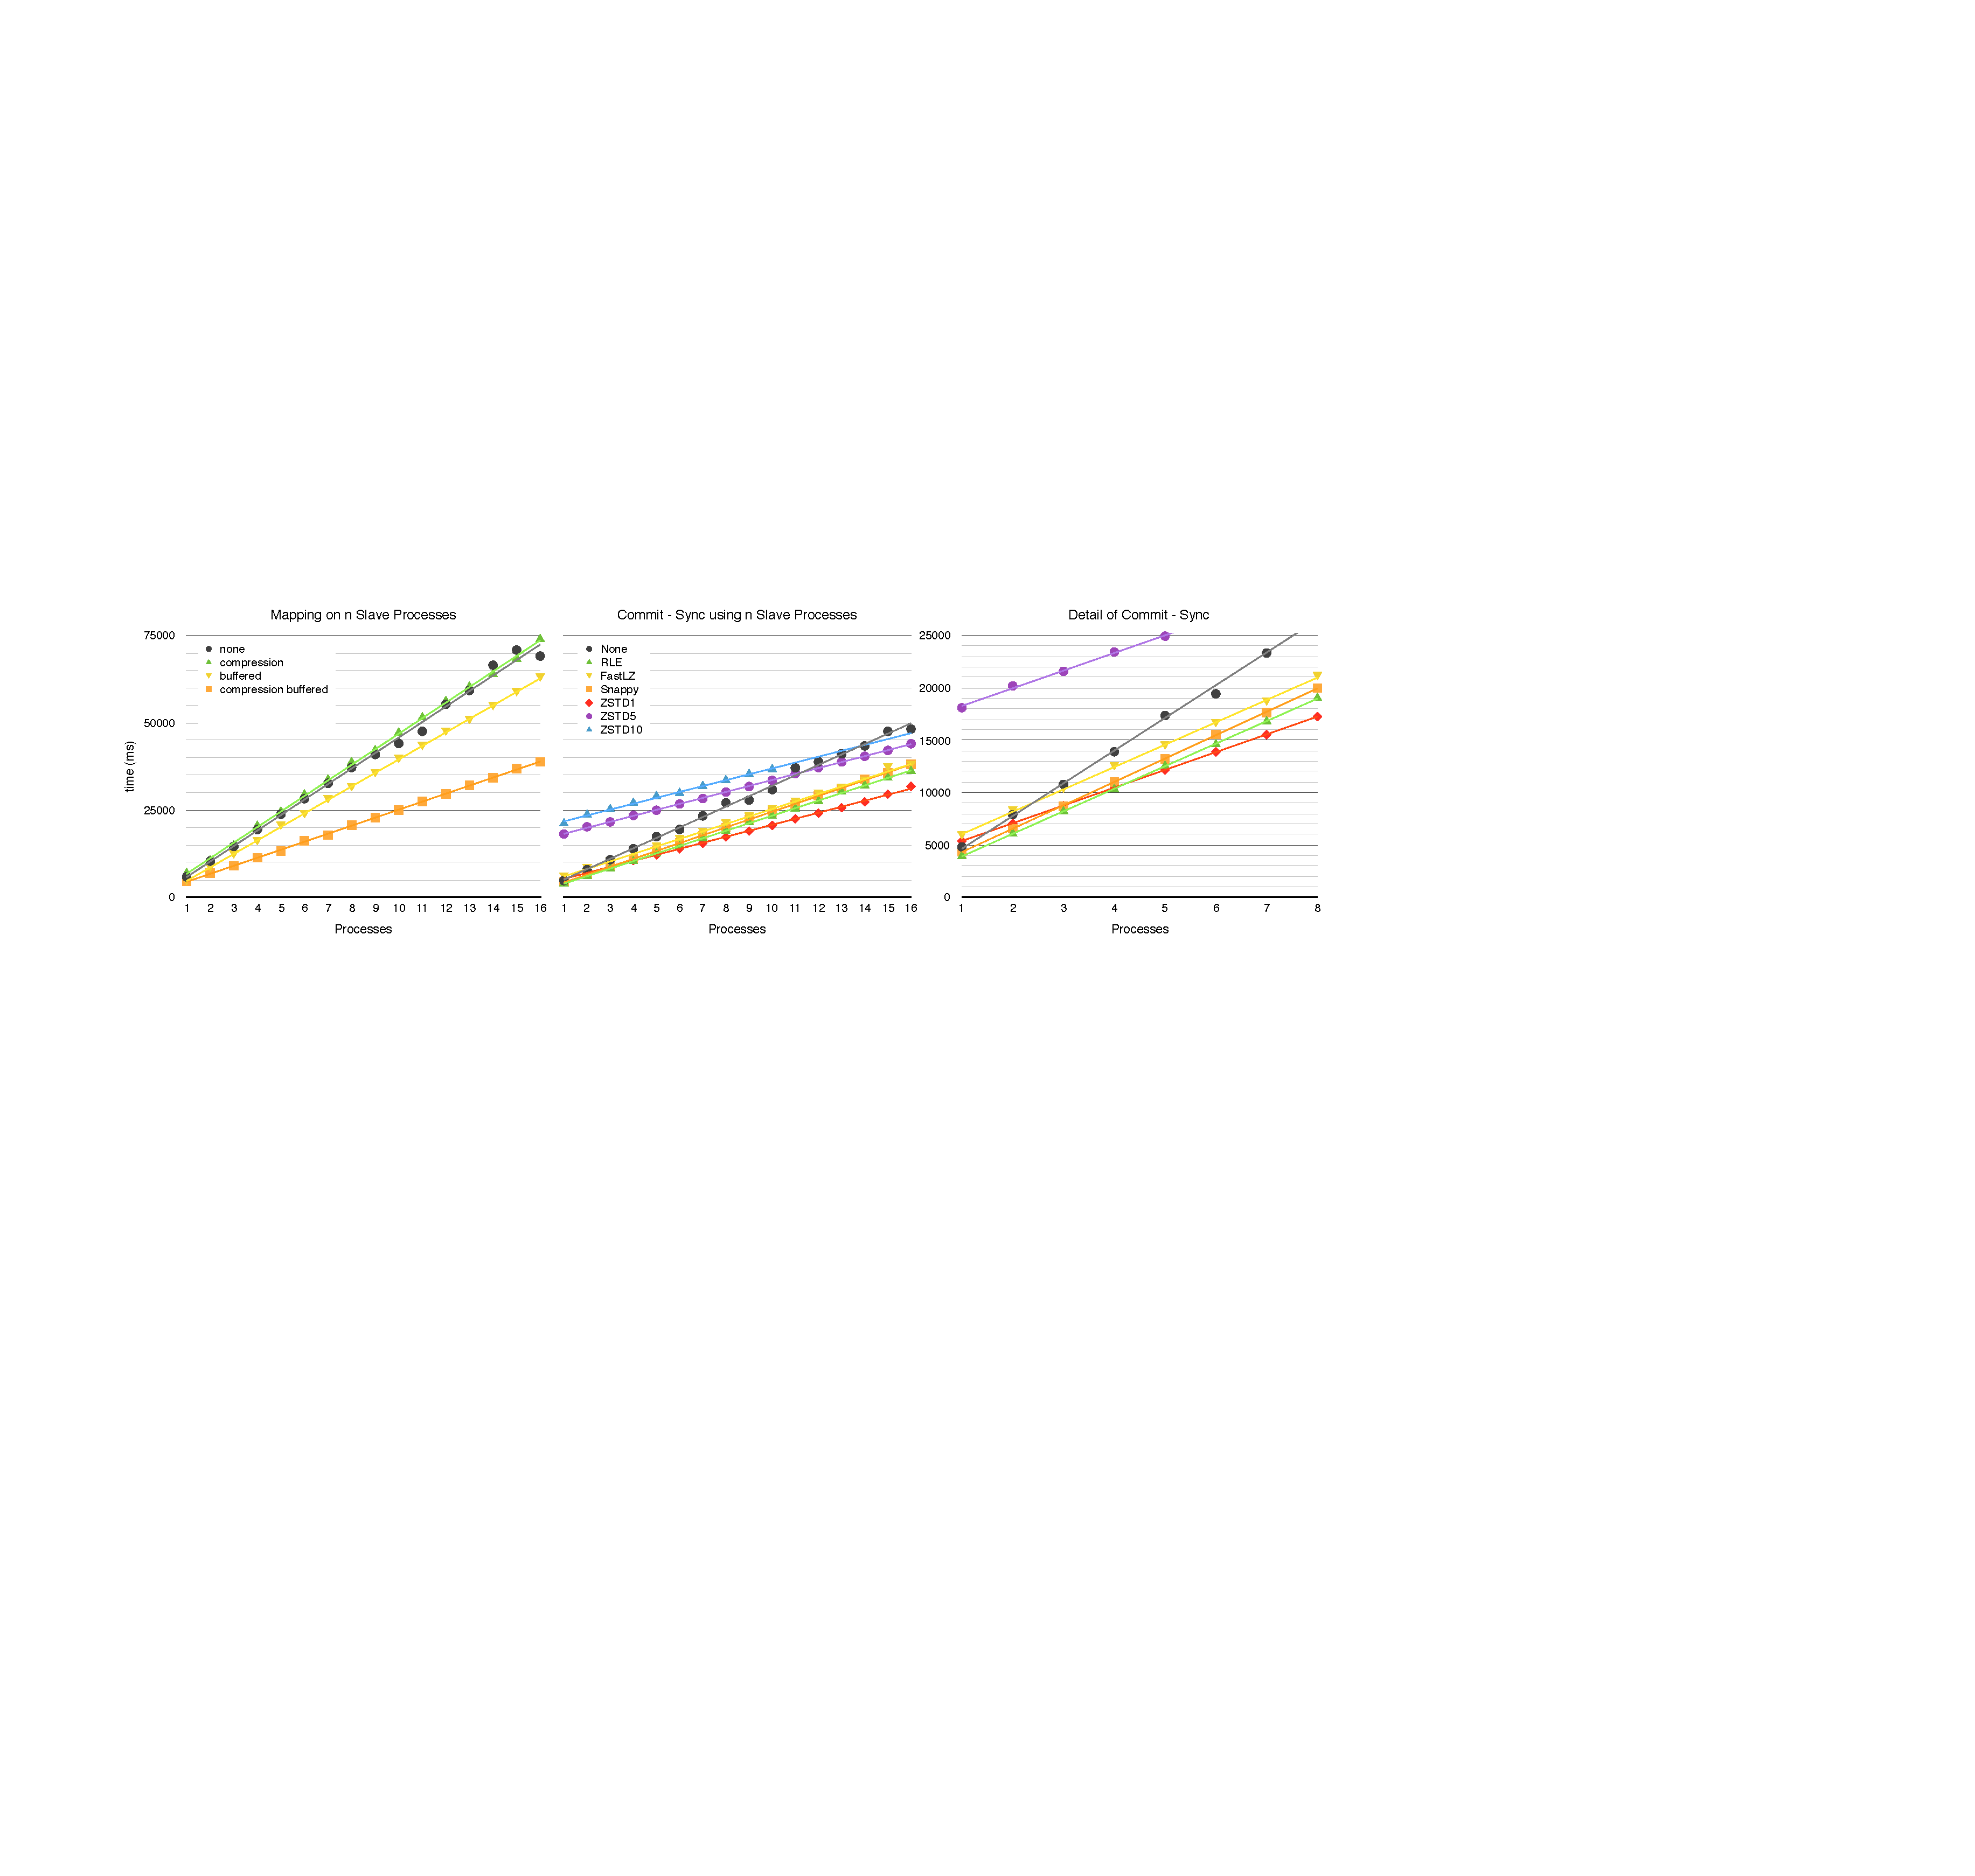
\includegraphics[height=.19\textheight]{images/beechnutdist}
  \caption{\label{fBeechnutDist}Object mapping (left) and data synchronization
    time (middle, detail view right) for the beechnut data set in
    \fig{fVolumes}, right}
\end{figure*}
\begin{figure*}[p!]\center
  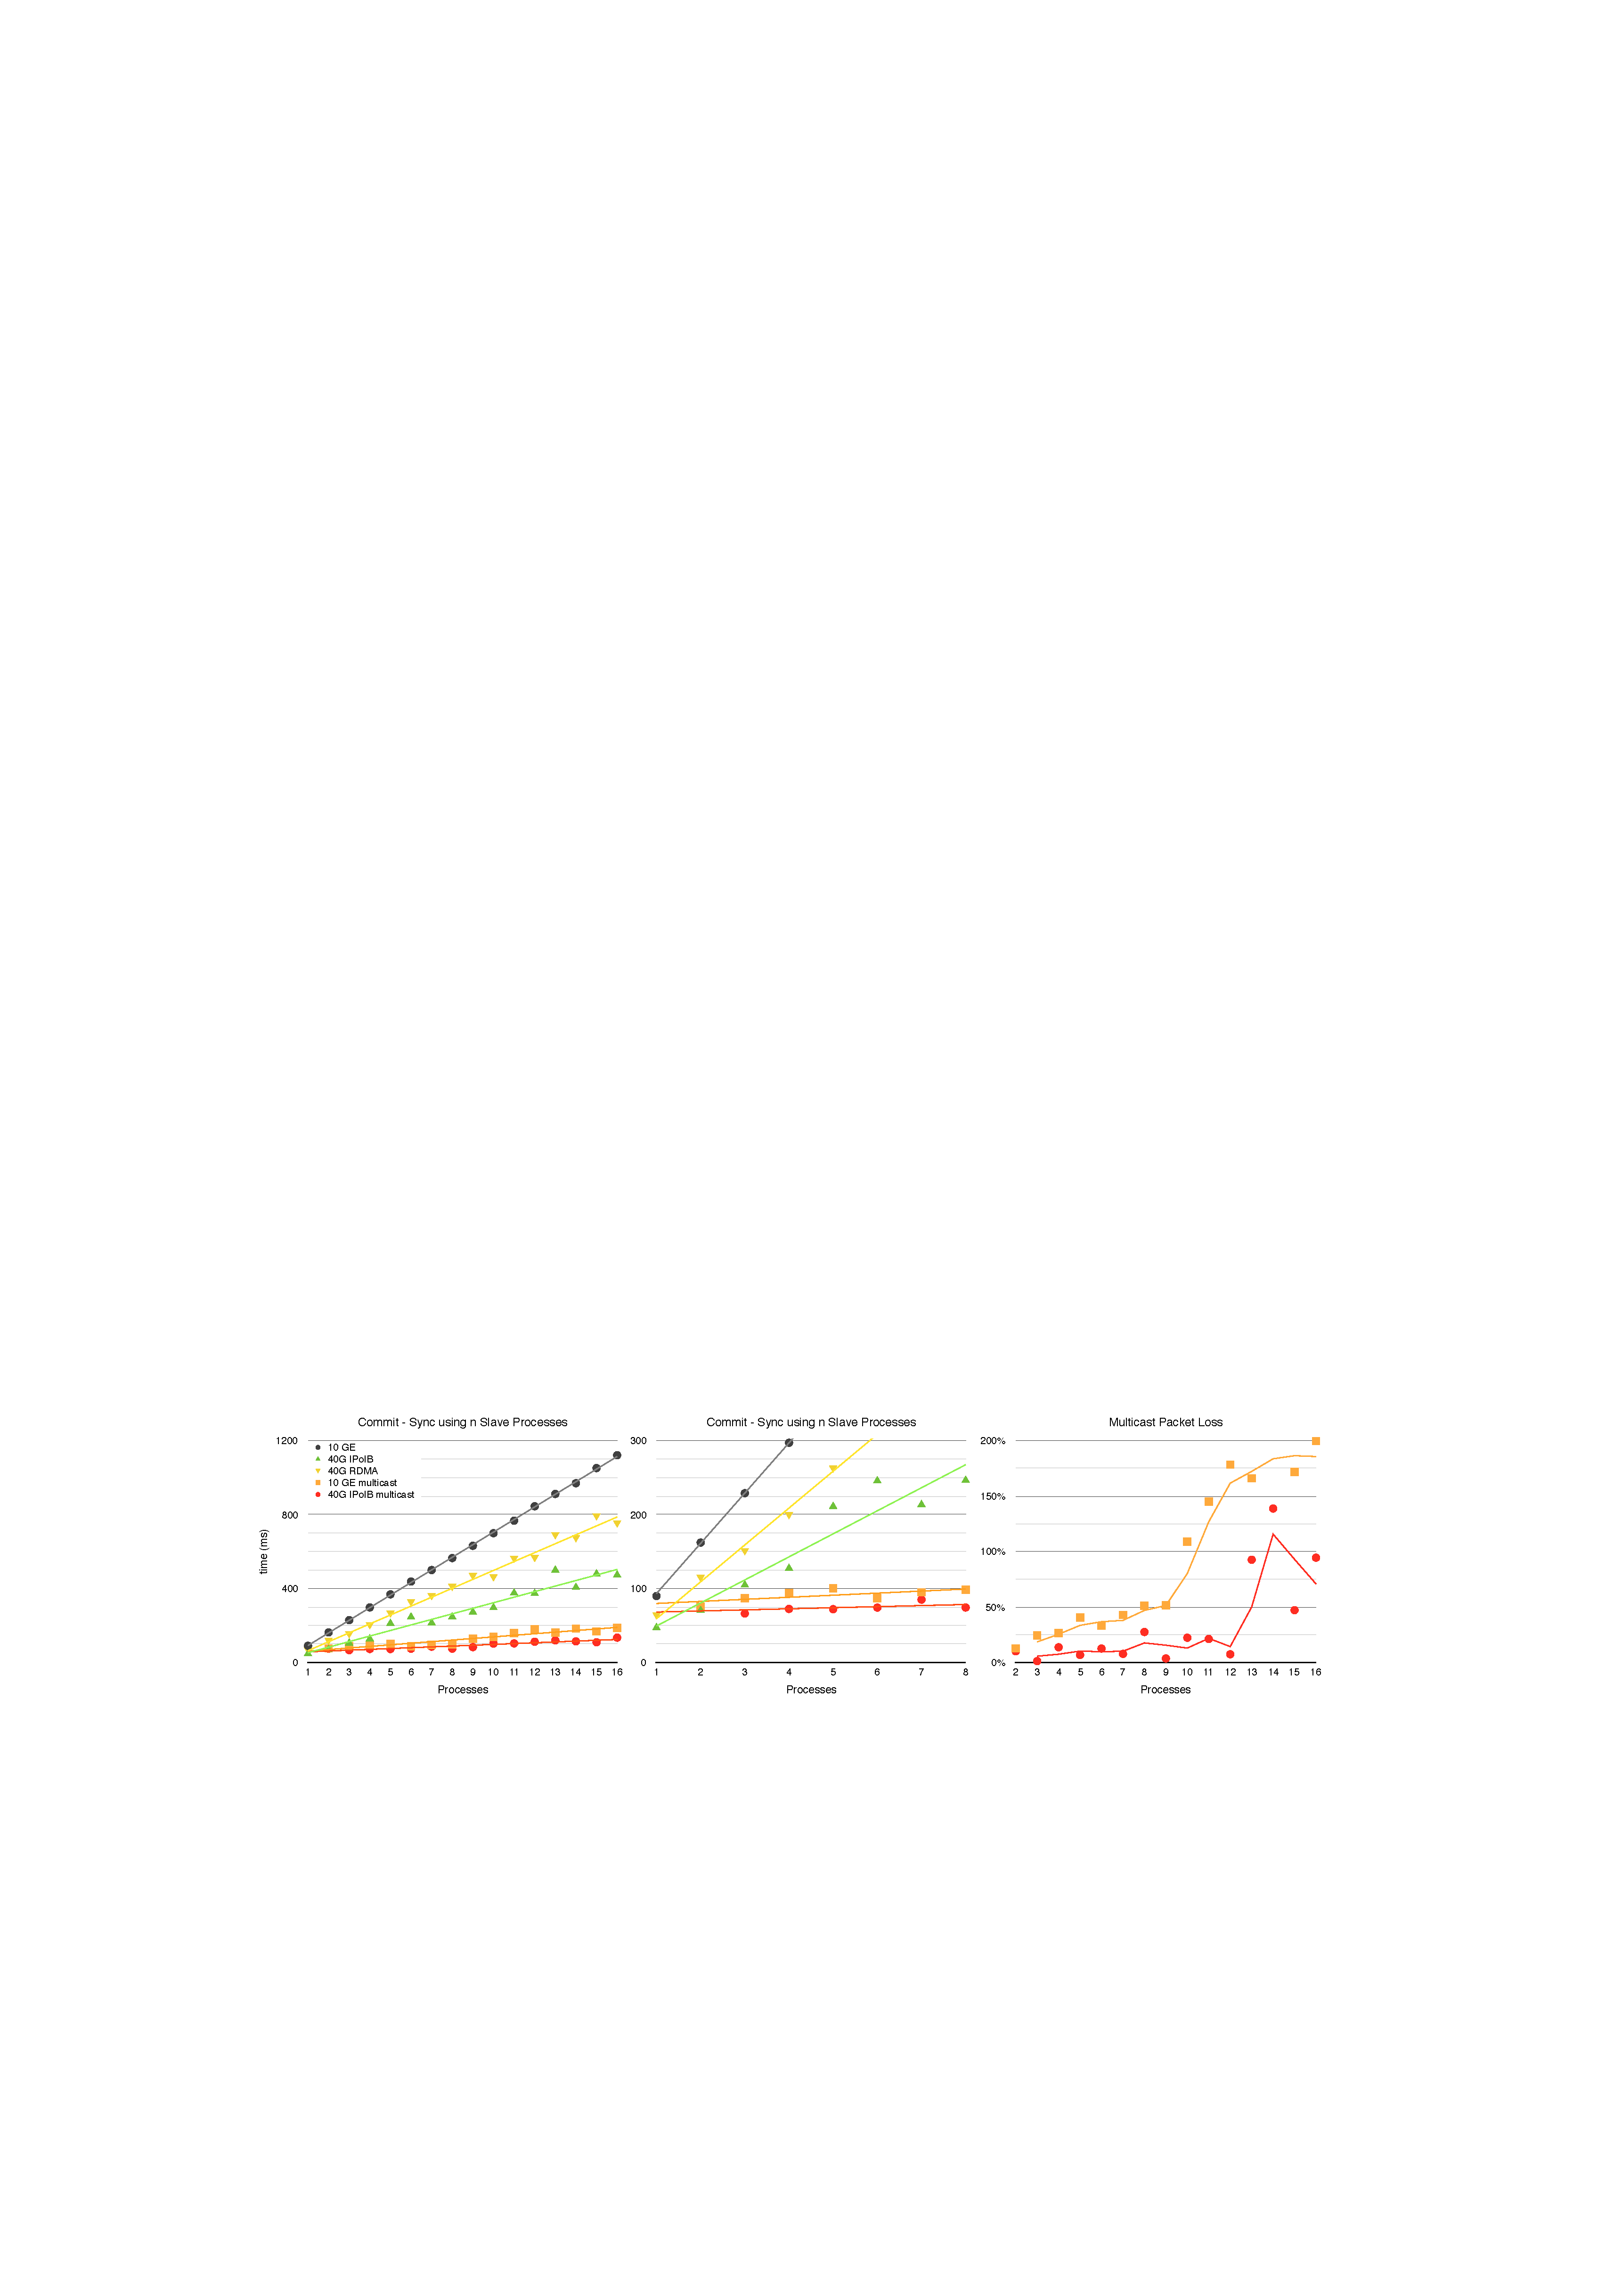
\includegraphics[height=.19\textheight]{images/ifdist}
  \caption{\label{fIFDist}Object synchronization using different network
    transports}
\end{figure*}

% that's all folks
\end{document}
